
%% bare_conf_compsoc.tex
%% V1.4b
%% 2015/08/26
%% by Michael Shell
%% See:
%% http://www.michaelshell.org/
%% for current contact information.
%%
%% This is a skeleton file demonstrating the use of IEEEtran.cls
%% (requires IEEEtran.cls version 1.8b or later) with an IEEE Computer
%% Society conference paper.
%%
%% Support sites:
%% http://www.michaelshell.org/tex/ieeetran/
%% http://www.ctan.org/pkg/ieeetran
%% and
%% http://www.ieee.org/

%%*************************************************************************
%% Legal Notice:
%% This code is offered as-is without any warranty either expressed or
%% implied; without even the implied warranty of MERCHANTABILITY or
%% FITNESS FOR A PARTICULAR PURPOSE! 
%% User assumes all risk.
%% In no event shall the IEEE or any contributor to this code be liable for
%% any damages or losses, including, but not limited to, incidental,
%% consequential, or any other damages, resulting from the use or misuse
%% of any information contained here.
%%
%% All comments are the opinions of their respective authors and are not
%% necessarily endorsed by the IEEE.
%%
%% This work is distributed under the LaTeX Project Public License (LPPL)
%% ( http://www.latex-project.org/ ) version 1.3, and may be freely used,
%% distributed and modified. A copy of the LPPL, version 1.3, is included
%% in the base LaTeX documentation of all distributions of LaTeX released
%% 2003/12/01 or later.
%% Retain all contribution notices and credits.
%% ** Modified files should be clearly indicated as such, including  **
%% ** renaming them and changing author support contact information. **
%%*************************************************************************


% *** Authors should verify (and, if needed, correct) their LaTeX system  ***
% *** with the testflow diagnostic prior to trusting their LaTeX platform ***
% *** with production work. The IEEE's font choices and paper sizes can   ***
% *** trigger bugs that do not appear when using other class files.       ***                          ***
% The testflow support page is at:
% http://www.michaelshell.org/tex/testflow/



\documentclass[conference,compsoc]{IEEEtran}
% Some/most Computer Society conferences require the compsoc mode option,
% but others may want the standard conference format.
%
% If IEEEtran.cls has not been installed into the LaTeX system files,
% manually specify the path to it like:
% \documentclass[conference,compsoc]{../sty/IEEEtran}





% Some very useful LaTeX packages include:
% (uncomment the ones you want to load)


% *** MISC UTILITY PACKAGES ***
%
%\usepackage{ifpdf}
% Heiko Oberdiek's ifpdf.sty is very useful if you need conditional
% compilation based on whether the output is pdf or dvi.
% usage:
% \ifpdf
%   % pdf code
% \else
%   % dvi code
% \fi
% The latest version of ifpdf.sty can be obtained from:
% http://www.ctan.org/pkg/ifpdf
% Also, note that IEEEtran.cls V1.7 and later provides a builtin
% \ifCLASSINFOpdf conditional that works the same way.
% When switching from latex to pdflatex and vice-versa, the compiler may
% have to be run twice to clear warning/error messages.
\usepackage{hyperref}

\usepackage{bm}

\usepackage{amsmath}

% *** CITATION PACKAGES ***
%
\ifCLASSOPTIONcompsoc
  % IEEE Computer Society needs nocompress option
  % requires cite.sty v4.0 or later (November 2003)
  \usepackage[nocompress]{cite}
\else
  % normal IEEE
  \usepackage{cite}
\fi
% cite.sty was written by Donald Arseneau
% V1.6 and later of IEEEtran pre-defines the format of the cite.sty package
% \cite{} output to follow that of the IEEE. Loading the cite package will
% result in citation numbers being automatically sorted and properly
% "compressed/ranged". e.g., [1], [9], [2], [7], [5], [6] without using
% cite.sty will become [1], [2], [5]--[7], [9] using cite.sty. cite.sty's
% \cite will automatically add leading space, if needed. Use cite.sty's
% noadjust option (cite.sty V3.8 and later) if you want to turn this off
% such as if a citation ever needs to be enclosed in parenthesis.
% cite.sty is already installed on most LaTeX systems. Be sure and use
% version 5.0 (2009-03-20) and later if using hyperref.sty.
% The latest version can be obtained at:
% http://www.ctan.org/pkg/cite
% The documentation is contained in the cite.sty file itself.
%
% Note that some packages require special options to format as the Computer
% Society requires. In particular, Computer Society  papers do not use
% compressed citation ranges as is done in typical IEEE papers
% (e.g., [1]-[4]). Instead, they list every citation separately in order
% (e.g., [1], [2], [3], [4]). To get the latter we need to load the cite
% package with the nocompress option which is supported by cite.sty v4.0
% and later.

%----------------------------------------------------------------------------------------------------------------
\usepackage{etoolbox}
\makeatletter
\patchcmd{\@makecaption}
  {\scshape}
  {}
  {}
  {}
\makeatother
\def\tablename{Table}

%---------------------------------------------------------------------------------------------------------------



% *** GRAPHICS RELATED PACKAGES ***
%
\ifCLASSINFOpdf
   \usepackage[pdftex]{graphicx}
  % declare the path(s) where your graphic files are
   \graphicspath{{/Users/JohnsonJohnson/Downloads/ReIDCodes/Figures/}{../pdf/}{../jpeg/}}
  % and their extensions so you won't have to specify these with
  % every instance of \includegraphics
   \DeclareGraphicsExtensions{.pdf,.jpeg,.png}
\else
  % or other class option (dvipsone, dvipdf, if not using dvips). graphicx
  % will default to the driver specified in the system graphics.cfg if no
  % driver is specified.
  % \usepackage[dvips]{graphicx}
  % declare the path(s) where your graphic files are
  % \graphicspath{{../eps/}}
  % and their extensions so you won't have to specify these with
  % every instance of \includegraphics
  % \DeclareGraphicsExtensions{.eps}
\fi
% graphicx was written by David Carlisle and Sebastian Rahtz. It is
% required if you want graphics, photos, etc. graphicx.sty is already
% installed on most LaTeX systems. The latest version and documentation
% can be obtained at: 
% http://www.ctan.org/pkg/graphicx
% Another good source of documentation is "Using Imported Graphics in
% LaTeX2e" by Keith Reckdahl which can be found at:
% http://www.ctan.org/pkg/epslatex
%
% latex, and pdflatex in dvi mode, support graphics in encapsulated
% postscript (.eps) format. pdflatex in pdf mode supports graphics
% in .pdf, .jpeg, .png and .mps (metapost) formats. Users should ensure
% that all non-photo figures use a vector format (.eps, .pdf, .mps) and
% not a bitmapped formats (.jpeg, .png). The IEEE frowns on bitmapped formats
% which can result in "jaggedy"/blurry rendering of lines and letters as
% well as large increases in file sizes.
%
% You can find documentation about the pdfTeX application at:
% http://www.tug.org/applications/pdftex





% *** MATH PACKAGES ***
%
%\usepackage{amsmath}
% A popular package from the American Mathematical Society that provides
% many useful and powerful commands for dealing with mathematics.
%
% Note that the amsmath package sets \interdisplaylinepenalty to 10000
% thus preventing page breaks from occurring within multiline equations. Use:
%\interdisplaylinepenalty=2500
% after loading amsmath to restore such page breaks as IEEEtran.cls normally
% does. amsmath.sty is already installed on most LaTeX systems. The latest
% version and documentation can be obtained at:
% http://www.ctan.org/pkg/amsmath





% *** SPECIALIZED LIST PACKAGES ***
%
%\usepackage{algorithmic}
% algorithmic.sty was written by Peter Williams and Rogerio Brito.
% This package provides an algorithmic environment fo describing algorithms.
% You can use the algorithmic environment in-text or within a figure
% environment to provide for a floating algorithm. Do NOT use the algorithm
% floating environment provided by algorithm.sty (by the same authors) or
% algorithm2e.sty (by Christophe Fiorio) as the IEEE does not use dedicated
% algorithm float types and packages that provide these will not provide
% correct IEEE style captions. The latest version and documentation of
% algorithmic.sty can be obtained at:
% http://www.ctan.org/pkg/algorithms
% Also of interest may be the (relatively newer and more customizable)
% algorithmicx.sty package by Szasz Janos:
% http://www.ctan.org/pkg/algorithmicx

\usepackage{float}
\usepackage[numbers,sort&compress]{natbib} %cite several papers in a \cite

% *** ALIGNMENT PACKAGES ***
%
%\usepackage{array}
% Frank Mittelbach's and David Carlisle's array.sty patches and improves
% the standard LaTeX2e array and tabular environments to provide better
% appearance and additional user controls. As the default LaTeX2e table
% generation code is lacking to the point of almost being broken with
% respect to the quality of the end results, all users are strongly
% advised to use an enhanced (at the very least that provided by array.sty)
% set of table tools. array.sty is already installed on most systems. The
% latest version and documentation can be obtained at:
% http://www.ctan.org/pkg/array


% IEEEtran contains the IEEEeqnarray family of commands that can be used to
% generate multiline equations as well as matrices, tables, etc., of high
% quality.




% *** SUBFIGURE PACKAGES ***
%\ifCLASSOPTIONcompsoc
%  \usepackage[caption=false,font=footnotesize,labelfont=sf,textfont=sf]{subfig}
%\else
%  \usepackage[caption=false,font=footnotesize]{subfig}
%\fi
% subfig.sty, written by Steven Douglas Cochran, is the modern replacement
% for subfigure.sty, the latter of which is no longer maintained and is
% incompatible with some LaTeX packages including fixltx2e. However,
% subfig.sty requires and automatically loads Axel Sommerfeldt's caption.sty
% which will override IEEEtran.cls' handling of captions and this will result
% in non-IEEE style figure/table captions. To prevent this problem, be sure
% and invoke subfig.sty's "caption=false" package option (available since
% subfig.sty version 1.3, 2005/06/28) as this is will preserve IEEEtran.cls
% handling of captions.
% Note that the Computer Society format requires a sans serif font rather
% than the serif font used in traditional IEEE formatting and thus the need
% to invoke different subfig.sty package options depending on whether
% compsoc mode has been enabled.
%
% The latest version and documentation of subfig.sty can be obtained at:
% http://www.ctan.org/pkg/subfig




% *** FLOAT PACKAGES ***
%
%\usepackage{fixltx2e}
% fixltx2e, the successor to the earlier fix2col.sty, was written by
% Frank Mittelbach and David Carlisle. This package corrects a few problems
% in the LaTeX2e kernel, the most notable of which is that in current
% LaTeX2e releases, the ordering of single and double column floats is not
% guaranteed to be preserved. Thus, an unpatched LaTeX2e can allow a
% single column figure to be placed prior to an earlier double column
% figure.
% Be aware that LaTeX2e kernels dated 2015 and later have fixltx2e.sty's
% corrections already built into the system in which case a warning will
% be issued if an attempt is made to load fixltx2e.sty as it is no longer
% needed.
% The latest version and documentation can be found at:
% http://www.ctan.org/pkg/fixltx2e


%\usepackage{stfloats}
% stfloats.sty was written by Sigitas Tolusis. This package gives LaTeX2e
% the ability to do double column floats at the bottom of the page as well
% as the top. (e.g., "\begin{figure*}[!b]" is not normally possible in
% LaTeX2e). It also provides a command:
%\fnbelowfloat
% to enable the placement of footnotes below bottom floats (the standard
% LaTeX2e kernel puts them above bottom floats). This is an invasive package
% which rewrites many portions of the LaTeX2e float routines. It may not work
% with other packages that modify the LaTeX2e float routines. The latest
% version and documentation can be obtained at:
% http://www.ctan.org/pkg/stfloats
% Do not use the stfloats baselinefloat ability as the IEEE does not allow
% \baselineskip to stretch. Authors submitting work to the IEEE should note
% that the IEEE rarely uses double column equations and that authors should try
% to avoid such use. Do not be tempted to use the cuted.sty or midfloat.sty
% packages (also by Sigitas Tolusis) as the IEEE does not format its papers in
% such ways.
% Do not attempt to use stfloats with fixltx2e as they are incompatible.
% Instead, use Morten Hogholm'a dblfloatfix which combines the features
% of both fixltx2e and stfloats:
%
% \usepackage{dblfloatfix}
% The latest version can be found at:
% http://www.ctan.org/pkg/dblfloatfix




% *** PDF, URL AND HYPERLINK PACKAGES ***
%
%\usepackage{url}
% url.sty was written by Donald Arseneau. It provides better support for
% handling and breaking URLs. url.sty is already installed on most LaTeX
% systems. The latest version and documentation can be obtained at:
% http://www.ctan.org/pkg/url
% Basically, \url{my_url_here}.




% *** Do not adjust lengths that control margins, column widths, etc. ***
% *** Do not use packages that alter fonts (such as pslatex).         ***
% There should be no need to do such things with IEEEtran.cls V1.6 and later.
% (Unless specifically asked to do so by the journal or conference you plan
% to submit to, of course. )


% correct bad hyphenation here
\hyphenation{op-tical net-works semi-conduc-tor}


\begin{document}
%
% paper title
% Titles are generally capitalized except for words such as a, an, and, as,
% at, but, by, for, in, nor, of, on, or, the, to and up, which are usually
% not capitalized unless they are the first or last word of the title.
% Linebreaks \\ can be used within to get better formatting as desired.
% Do not put math or special symbols in the title.
\title{Person re-identification based on and kernel local fisher discriminant analysis and Mahanalobis distance learning}


% author names and affiliations
% use a multiple column layout for up to three different
% affiliations
\author{\IEEEauthorblockN{Qiangsen He}
\IEEEauthorblockA{School of Electrical Engineering and Computer Science,
University of Ottawa\\
Ottawa, Ontario,
qiangsenhe@gmail.com}

%\and
%\IEEEauthorblockN{Homer Simpson}
%\IEEEauthorblockA{Twentieth Century Fox\\
%Springfield, USA\\
%Email: homer@thesimpsons.com}
%\and
%\IEEEauthorblockN{James Kirk\\ and Montgomery Scott}
%\IEEEauthorblockA{Starfleet Academy\\
%San Francisco, California 96678-2391\\
%Telephone: (800) 555--1212\\
%Fax: (888) 555--1212}}
}

% conference papers do not typically use \thanks and this command
% is locked out in conference mode. If really needed, such as for
% the acknowledgment of grants, issue a \IEEEoverridecommandlockouts
% after \documentclass

% for over three affiliations, or if they all won't fit within the width
% of the page (and note that there is less available width in this regard for
% compsoc conferences compared to traditional conferences), use this
% alternative format:
% 
%\author{\IEEEauthorblockN{Michael Shell\IEEEauthorrefmark{1},
%Homer Simpson\IEEEauthorrefmark{2},
%James Kirk\IEEEauthorrefmark{3}, 
%Montgomery Scott\IEEEauthorrefmark{3} and
%Eldon Tyrell\IEEEauthorrefmark{4}}
%\IEEEauthorblockA{\IEEEauthorrefmark{1}School of Electrical and Computer Engineering\\
%Georgia Institute of Technology,
%Atlanta, Georgia 30332--0250\\ Email: see http://www.michaelshell.org/contact.html}
%\IEEEauthorblockA{\IEEEauthorrefmark{2}Twentieth Century Fox, Springfield, USA\\
%Email: homer@thesimpsons.com}
%\IEEEauthorblockA{\IEEEauthorrefmark{3}Starfleet Academy, San Francisco, California 96678-2391\\
%Telephone: (800) 555--1212, Fax: (888) 555--1212}
%\IEEEauthorblockA{\IEEEauthorrefmark{4}Tyrell Inc., 123 Replicant Street, Los Angeles, California 90210--4321}}




% use for special paper notices
%\IEEEspecialpapernotice{(Invited Paper)}




% make the title area
\maketitle

% As a general rule, do not put math, special symbols or citations
% in the abstract
\begin{abstract}

In person re-identification(re-ID) it's very important to choose robust descriptors and metric learning to improve accuracy. Mahanalobis distance based metric learning is a popular method for metric learning. However, since directly extracted descriptors usually have high dimension(thousands or more), it's intractable to learn a high dimensional semi-definite positive(SPD) matrix without dimension reduction.  Many subspace learning metrics have been proposed to learn a subspace while preserving those discriminative information as much as possible. However, few work has been done to probe the metric learning on those subspace after the first-time metric learning. In this paper the KLFDA \cite{KLFDA} is used to reduce dimension given that kernelization method can greatly improve re-identification performance for nonlinearity. Then a Mahanalobis distance metric is learned on lower dimensional descriptors based on the limitation that the intraclass distance is at least 1 unit smaller than the minimum interclass distance. By comparing the intraclass distance only with the interclass distance the computation complexity is reduced. This method turns to have excellent performance compared with other advanced metric learning.


%In this paper a new descriptor based on hierarchical gaussian distribution of pixel feature is proposed.
%There are a few steps for this algorithm. First, the image is segmented into many super pixels patches.
%Then for each super pixel a gaussian distribution describing its pixel feature distributions.  The result of gaussian 
%model is the mean value and covariance matrix of the super pixel patch. Through a Riemannian manifold transformation,
%the mean value vector and covariance matrix can be merged into a matrix with higher dimension.  Since this matrix is a 
%symmetric matrix, we extract its upper triangle part and reshape it to be a vector. Secondly, when all the gaussian distribution 
%of super pixels are computed, we model all the patches with another gaussian model(or GMM), with the same process 
%the mean and covariance matrix is transformed into a vector. By comparing this descriptor we find it has state-of-the-art performance
%on those main re-ID datasets.
\end{abstract}

% no keywords




% For peer review papers, you can put extra information on the cover
% page as needed:
% \ifCLASSOPTIONpeerreview
% \begin{center} \bfseries EDICS Category: 3-BBND \end{center}
% \fi
%
% For peerreview papers, this IEEEtran command inserts a page break and
% creates the second title. It will be ignored for other modes.
\IEEEpeerreviewmaketitle



\section{Introduction}
% no \IEEEPARstart
Person re-identification(re-ID) has received increasing attention in recent years. This task is very challenging caused by many factors like low image resolution, occlusion, background noise and different camera color response, etc. In the single shot re-ID problem, since only one image is provided in each camera for each person, it might be quite confusing when different people have similar pose or clothes. Also, in the multi-shots case, there might exist quite much difference even in different frames of the same person for different pose and illuminations \cite{TDL}. Therefore, good descriptors are supposed to be robust to illumination change and occlusions.

% -------the descriptor part
Most previous work try to find better feature representation \cite{LOMO, GOG, RegionCovariance, SDALF} and metric learning \cite{KISSME, LFDA, PCCA, TDL, PRDC, LMNN, KLFDA, KCCA, KernelVersionMetrics, NFST, ITML}, or a subspace learning. Most descriptors are color and texture based descriptors. Distance metric learning has been fully studied in \cite{MetricSurvey}, most existing metric learning are based on Mahanalobis distance to learn a metric which outputs small intraclass distance and large interclass distance. Though much progress has been made, there still exists some challenges caused by classical problems like small sample problem(SSS), computation complexity on large datasets. 
%Metric learning 
\indent Among all those metric learning methods, fisher discriminant analysis(FDA) proves to be one of advanced metrics to improve re-ID performance. It tries to maximize the ration of interclass scatter matrix versus intraclass scatter distance and this problem is transformed as a eigenvalue decomposition problem. Local fisher discriminant analysis combines locality preserving projection(LPP) with FDA to exploit locality of sample points. Besides, kernel method \cite{KernelVersionMetrics} has been shown to improve re-ID performance since it exploits the nonlinearity of data.\\
\indent For descriptors with high dimension($d\ge1000$), it's hard to directly learn a Mahanalobis distance matrix $M$ for the small sample size $n(n<<d)$. A popular method is to use principal component analysis(PCA) to reduce dimension. PCA is a very popular preprocessing method which uses an orthogonal transformation to convert a set of observations of possibly correlated variables into a set of values of linearly uncorrelated variables called principal components. One problem is  PCA doesn't consider the information between classes thus many discriminant information will be lost after dimension reduction. In this paper kernel local fisher discriminant Analysis(KLFDA) \cite{KLFDA} is used to reduce dimension, this supervised dimension reduction combines the linear discriminant analysis and locality preserving projection. Moreover, the kernelization version of LFDA proves to improve performance and reduce computation cost. However, the metric learning on dimension reduced vectors by KLFDA hasn't been fully probed.\\
\indent In this paper, KLFDA is only used to reduce dimension instead of being used as an unique subspace learning method. Previous work uses Euclidean distance to measure the similarity after dimension reduction with KLFDA, and the metric learning on the projected vector space by KLFDA has not been fully probed. In this paper for the dimension reduced data, a Mahanalobis distance matrix $M$ is learned based on the limitation that intra distance is at least 1 unit smaller than interclass distance. This iterative metric learning method is inspired by the \cite{TDL} paper. A target function respect $M$ is created to penalize big intraclass distance and small interclass distance. So we transformed re-ID into a optimization problem in the lower dimension space. With the target function, the gradient descent method is used to get a optimal $M$.


%There are a few differences between LDA and PCA, LDA is a supervised method while PCA is unsupervised, and LDA is more used independently while PCA is more used as a preprocessing method. The advantage of LDA is it distinguishes different classes by maximize the ratio of inter-class scatter matrix versus intra-class scatter matrix. 
 %The local fisher discriminant analysis(LDFA) combines LDA and locality projection preserving(LPP) to exploit the locality of sample points.  

% You must have at least 2 lines in the paragraph with the drop letter
% (should never be an issue)


%\hfill mds
%
%\hfill August 26, 2015

%\subsection{Subsection Heading Here}
%Subsection text here.
%
%
%\subsubsection{Subsubsection Heading Here}
%Subsubsection text here.


% An example of a floating figure using the graphicx package.
% Note that \label must occur AFTER (or within) \caption.
% For figures, \caption should occur after the \includegraphics.
% Note that IEEEtran v1.7 and later has special internal code that
% is designed to preserve the operation of \label within \caption
% even when the captionsoff option is in effect. However, because
% of issues like this, it may be the safest practice to put all your
% \label just after \caption rather than within \caption{}.
%
% Reminder: the "draftcls" or "draftclsnofoot", not "draft", class
% option should be used if it is desired that the figures are to be
% displayed while in draft mode.
%
%\begin{figure}[!t]
%\centering
%\includegraphics[width=2.5in]{myfigure}
% where an .eps filename suffix will be assumed under latex, 
% and a .pdf suffix will be assumed for pdflatex; or what has been declared
% via \DeclareGraphicsExtensions.
%\caption{Simulation results for the network.}
%\label{fig_sim}
%\end{figure}

% Note that the IEEE typically puts floats only at the top, even when this
% results in a large percentage of a column being occupied by floats.


% An example of a double column floating figure using two subfigures.
% (The subfig.sty package must be loaded for this to work.)
% The subfigure \label commands are set within each subfloat command,
% and the \label for the overall figure must come after \caption.
% \hfil is used as a separator to get equal spacing.
% Watch out that the combined width of all the subfigures on a 
% line do not exceed the text width or a line break will occur.
%
%\begin{figure*}[!t]
%\centering
%\subfloat[Case I]{\includegraphics[width=2.5in]{box}%
%\label{fig_first_case}}
%\hfil
%\subfloat[Case II]{\includegraphics[width=2.5in]{box}%
%\label{fig_second_case}}
%\caption{Simulation results for the network.}
%\label{fig_sim}
%\end{figure*}
%
% Note that often IEEE papers with subfigures do not employ subfigure
% captions (using the optional argument to \subfloat[]), but instead will
% reference/describe all of them (a), (b), etc., within the main caption.
% Be aware that for subfig.sty to generate the (a), (b), etc., subfigure
% labels, the optional argument to \subfloat must be present. If a
% subcaption is not desired, just leave its contents blank,
% e.g., \subfloat[].


% An example of a floating table. Note that, for IEEE style tables, the
% \caption command should come BEFORE the table and, given that table
% captions serve much like titles, are usually capitalized except for words
% such as a, an, and, as, at, but, by, for, in, nor, of, on, or, the, to
% and up, which are usually not capitalized unless they are the first or
% last word of the caption. Table text will default to \footnotesize as
% the IEEE normally uses this smaller font for tables.
% The \label must come after \caption as always.
%
%\begin{table}[!t]
%% increase table row spacing, adjust to taste
%\renewcommand{\arraystretch}{1.3}
% if using array.sty, it might be a good idea to tweak the value of
% \extrarowheight as needed to properly center the text within the cells
%\caption{An Example of a Table}
%\label{table_example}
%\centering
%% Some packages, such as MDW tools, offer better commands for making tables
%% than the plain LaTeX2e tabular which is used here.
%\begin{tabular}{|c||c|}
%\hline
%One & Two\\
%\hline
%Three & Four\\
%\hline
%\end{tabular}
%\end{table}


% Note that the IEEE does not put floats in the very first column
% - or typically anywhere on the first page for that matter. Also,
% in-text middle ("here") positioning is typically not used, but it
% is allowed and encouraged for Computer Society conferences (but
% not Computer Society journals). Most IEEE journals/conferences use
% top floats exclusively. 
% Note that, LaTeX2e, unlike IEEE journals/conferences, places
% footnotes above bottom floats. This can be corrected via the
% \fnbelowfloat command of the stfloats package.
\section{Related work}
%\subsection{Appearance descriptors}
Previous work focus on find more discriminative descriptors and better metric learning. A good descriptor is robust to problems like illumination, low resolution and viewpoint, etc. In \cite{SDALF} the symmetry and asymmetry property of pedestrian foreground is considered. But this descriptor depends much on foreground extraction performance. In \cite{ImportantFeat} the image is divided into a few horizontal strides, for each slide the color histogram is extracted, then the color histograms are concatenated together as the whole image's descriptor. This descriptor is simple but has low performance for it doesn't consider the texture and pixel spatial distribution. In \cite{RegionCovariance} the covariance descriptors of local patches are used to represent people. In \cite{LOMO} densely sampled overlapping small windows are adopted to overcome viewpoint variation. In each sample window the scale invariant local ternary pattern(SILTP) and local binary pattern(LBP) is extracted, then the local maximal occurrence of patterns of all windows are extracted to consist of LOMO descriptor. The LOMO descriptor succeeds in characterizing images with viewpoint changes. In \cite{GOG} a two-level multivariate gaussian descriptors are proposed to exploit the stochastic property of the color, texture. By a Riemannian manifold based mapping, this descriptors embeds $d$ dimensional multivariate gaussian function to a $d+1$ dimensional semi-positive definite space. Then by matrix vectorization we can get the gaussian of gaussian descriptor(GOG). The combination of GOG and cross view quadratic discriminative analysis outperforms most advanced works.

Other works try to use metric learning to improve re-ID performance. In \cite{PRDC} the distance between positive pairs must be smaller than the distance between negative pairs. Since it has to compare possible positive and negative pairs, computation complexity will be quite huge. In \cite{NFST} the author proposes to to learn a null space in which the descriptors of the same class will collapse into the same point while descriptors of different classed are projected onto different points. In \cite{MetricEnsembles} the author exploits the combination of different metrics by assigning weights to different metrics and optimize the weights to maximize probability that any of these top k matches are correct. In \cite{novelEMD} the author proposed a earth mover's distance(EMD) based metric learning for descriptors of gaussian mixture model(GMM). It's more complex to compute similarity of GMM model. However, one problem this EMD-based distance metric is it's huge time complexity, which limits its real-time application. In \cite{SemanticREID} the author presents a new semantic attribute learning approach for person re-identification and search but this method suffers from low performance. In \cite{LOMO} the author extends the Bayesian face and keep it simple and straightforward(KISSME) approaches to learn a discriminant low dimensional subspace by cross-view quadratic discriminant analysis(XQDA), this work has a top performance in most datasets when combined with LOMO descriptor and GOG descriptors. 

There are also some works which tries to use convolutional neural network \cite{PersonNetCNN,RecurrentCNN} to improve accuracy. However, person re-identification may be one of the area which CNN won't work for the small sample size(SSS) problem. In most datasets, the sample size of each pedestrian is quite small. Especially in single shot re-ID only one frame is provided in each view for each person. So re-ID will more rely on classical machine learning.

%
%With those equations above axis can be computed depend on specific image. This method has a relatively high performance.
%
%The part-based adaptive spatial-temporal model used in [7] characterizes person?s appearance using color and facial feature. Few work exploits human face feature but in this work human face selection based on low resolution cues selects useful face images to build face models. Color features capture representative color as well as the color distribution to build color model. This model handles multi-shots re-identification and it also model the color distribution variation of many consecutive frames.  Besides, the facial features of this model is conditional, that is, in the absence of good face images this model is only based on color features.
%
%Some methods based on learned part models have been proposed. Part model detectors, that is, statistic classifiers, are trained with manually labelled human body parts images, exploiting features related with edges contained in the images. The pictorial structure is proposed in [8], and a PS model of a non-rigid body is a collection of part models with deformable configurations and connections with certain parts. The appearance of each part is separately modelled and deformable configurations are implemented with spring-like connections. This model can quantitatively describe visual appearance and model the non-rigid body. In [8] the body model is made up of $N$ parts and $N$ corresponding part detectors. Suppose $L={(l_0,l_1,\ldots,_{N-1})}$ be the possible configurations of each part, where $l_i$ is the state of the i-th body part and $l_0=(x_i,y_i,\theta_i,s_i)$, $x_i$ and $y_i$ are the coordinates of the part center, $\theta_i$ is the absolute part orientation, and $s_i$ is the scale size relative to the part size in the training set.  Given the image evidence D, the problem is to maximize the posterior probability $P(D)$ that the part configuration is correct, and we have $P(D) \propto {P(L)*P(L)}$, where $P(L)$ is the likelihood of image evidence given a particular part configuration and P(L) corresponds to a kinematic prior, and those two items can be learned from a training set.
%
%Another example of learned part model is in [12,13], the overall human body model consists of several part models, each model is made up of a spatial model and a part filter. For each part the spatial model define allowed arrangements of this part with respect to the bounding box. To train each model the Latent Support Vector Machine is used and in [12,13 ] four body parts are detected, namely head, left and right torso and upper legs. Compared with other models this model exploits a sequence of frames of an individual and thus captures appearance characteristics as well as the appearance variation over time. 
%
%Moreover, 3-D model is proposed to improve re-ID performance. A new 3-D model model called SARC3D [16] is used to represent the individual. Compared with those 2-D models, this model combines the texture and color information with their location information together to get a 3D model. This model starts with an approximate body model with single shape parameter. By precise 3-D mapping this parameter can be learned and trained with even few images (even one image is feasible). This model?s construction is driven by the frontal, top and side views extracted from various videos, and for each view the silhouette of people is extracted to construct the 3-D graphical model. The final body model is sampled to get a set of vertices from previously learned graphic body model. Compared with other model, this model has a robust performance when dealing with partial occlusion, people pose and viewpoint variations since the model is based on people silhouettes from three viewpoints.
%
%As for the feature for each model (a whole model or part-based model), the feature can be implemented with different methods. The features can be divided into two categories, the global and local feature. The global feature refers to the feature extracted from a whole image or region, and the size of the descriptor is usually fixed. While to extract the local feature of a specified image or region, we first divide the whole image into many equal blocks and compute the feature of each block.  Both descriptors may deal with color, texture and shape. The color is exploited most as the color histogram within different color space. descriptor based on texture, such as the SIFT, SURF and LBP are also widely combined to improve the performance.
%
%Global color histogram is a frequently used global feature. For an three-channel image, like RGB image, each channel is quantized into $B$ bins separately. The final histogram could be a multi-dimensional or mono-dimensional histogram. For instance, if $B=8$, for multi-dimensional histogram there will be $8*8*8=512$ bins, but if we concatenate the 3 dimensional bins together the dimension can be reduced to $8+8+8=24$ bins while the performance of this reduced descriptor doesn't decrease. This method can be applied on other color spaces like HSV and Lab, etc.
%
%Local color histogram usually splits the specified model or region into many equal size blocks and compute the global feature of each block. The feature can be based on color, texture and interest points. SIFT[14] is a kind of local feature based on the interest points. The salient interest points (identifiable over rotating and scaling) are selected by the interest operator. This algorithm detects the scale-extrema of the function difference of Gaussian function with scale $\sigma$, that is, 
%$$D(x,y,\sigma) = (G(x,y,k_1\sigma)-G(x,y,k_2\sigma))*I(x,y)$$
%the Gaussian filter with standard deviation $k1*\sigma$, $I(x, y)$ is the image, when the DoG image is computed, each point $(x, y)$ is compared with its neighbours to get  extrema.
%
%
%RHSP (Recurrent Highly-Structured Patches) is used in [6]. This feature captures patches with highly recurrent color and texture characteristics from extracted silhouette pixels. This feature is extracted with following steps, first random and probably overlapping small image patches are extracted from silhouette pixels. Then to capture those patches with informative texture the entropy of each patch (the sum of three channels? entropy) is computed, we discard those patches with entropy smaller than a specified threshold. In the next step some transforms are performed on the remaining patches to select those remain invariant to the transforms. Subsequently, the recurrence of each patch is evaluated with the LNCC(local normalized cross correlation) function. This evaluation is only performed on small region containing the patch instead of the whole image. Then the patches with high recurrence is clustered to avoid patches with similar content. Finally, the Gaussian cluster is applied to maintain the patch nearest to cluster?s centroid for each cluster.
% 
%Combined descriptors are found to have better performance. Descriptors combining color and texture are most often used in re-identification. In [5] a signature called asymmetry-based histogram plus epitome(AHPE) was proposed. This work starts with a selection of images to reduce image redundancy (redundancy is caused by correlated consecutive sequences). This descriptor combines global and local statistical descriptors of human appearance, focusing on overall chromatic content via histogram and on the recurrent local patches via epitome analysis [6]. Similar to SDALF descriptor [6], HPE descriptor consists of three components, the chromatic color histogram, the generic epitome and local epitome. The chromatic color histogram is extracted in the HSV color space, which turns to be robust to illumination changes. Here color histogram is encoded into a 36-dimensional feature space $[H=16,  S=16,  V=4]$. Besides, the authors customize the use of epitome here by extracting generic and local epitome here. 
%
%%\subsection{Metric learning}
%The second step of re-ID is to design the similarity computing methodology to compare descriptors. That is, the way to compare how different two descriptors are. This is also call the metric learning. Generally, for two input vectors $x_1$, $x_2$, any symmetric positive demi-definite matrix W defines a pseudo-metric with the form of $D = x_1*W*x_2$. Many widely used distance metric obey this rule. Previous methods includes the Euclidean distance, Bhattacharyya distance and Mahalanobis distance. The Euclidean distance, which is mostly used for the straightforward descriptors like color and texture descriptors,  is one case of the $L_p$ distance when $p=2$, and also a special case of Mahalanobis distance when the covariance matrix of two input observations is an identity matrix. One example of metric learning is the probabilistic relative distance comparison model proposed in [4]. This model decreases the error caused by sometimes high intra-class variation and low inter-class variation. Compared with other distance learning models proposed, this model behaves more robust for its probability relative distance comparison model. Suppose z is an image of a person, the task is to identify another image $z'$ of the same person from $z''$ of a different person by using a distance model $f(.,.)$ so that $f(z, z')< f(z, z'')$. The contribution of this paper is that the author transfers the distance learning problem into a probability comparison problem by measuring the probability of distance between a relevant pair of images being smaller than that of a related irrelevant pair as
%\begin{equation}P(f(z,z')<f(z,z'')) = (1+e^{(f(z-z')-f(z-z''))})^{-1}\end{equation}
%Here the author assumes the probability of $f(z,z')$ and $f(z,z'')$ is independent, therefore, using maximal likelihood principal the optimal function can be learned as
%\begin{equation}
%\begin{aligned}
%f = \mathop{\arg\min}_f r(f,O) \\
%r(f,O) = -log(\Pi_{O_i}P(f(z-z')-f(z-z'')))
%\end{aligned}
%\end{equation}
%$O=\{O_i=(x_i^p-x_i^n)\}$ , $x_i^p$,$x_i^n$ are the pair from same person and different person respectively.
%The distance function $f(\cdot)$ here is parameterized as Mahalanobis distance function
%$f=\overrightarrow{x}^T\textbf{M}\overrightarrow{x},\textbf{M}\ge0$,
%here \textbf{M} is a semi-definite matrix, in this way the distance function learning problem is transformed to a matrix learning problem. The author used an iteration algorithm to compute matrix $M$.
%
%Since still image based person representation suffers from factors like illumination, occlusion, viewpoint change and pose difference. The multi-shot re-ID has been proposed. Since there are a sequence of images for each indivudual, there are much more cues to exploit.
%In [TDL], the author simplified computing of Mahananobis matrix by applying the new limitations on datasets. The author finds that when using video based person representation the difference of inter-class may be more obscure than that of still image based representation. Therefore, the author proposed the top-push distance learning. For a person video sequence, the maximal intra-class distance should be smaller than the minimal distance of inter-class distance. One another requirement is the sum of all intra-class distance should be as small as possible, so the final target function is summarized as 
%
%\begin{equation}
%\begin{aligned}
%f(D) = (1-\alpha)\sum_{x_i,x_j,y_i=y_j} D(x_i,x_j) + \\ \alpha \sum_{x_i,x_j,y_i=y_j}\max\{{D(x_i,x_j)-\min_{y_i\ne y_k}{D(x_i,x_k)}+\rho,0}\}
%\end{aligned}
%\end{equation}
%
%Cross view quadratic analysis(XQDA) is proposed in [xqda paper]. In [36 of lomo paper] Mogaddam et al. proposed to model each of two classes with a multivariate Gaussian  distribution. Suppose the sample difference $\Delta = x_i - x_j$, where $x_i$ and $x_j$ are two feature vectors. $\Delta$ is called intrapersonal difference when their label $y_i = y_j$ and extrapersonal difference when $y_i \ne y_j$. Respectively two the intrapersonal and interpersonal variation can be defined as $\Omega_I$ and $\Omega_E$,
%
%
%Besides those aforementioned metric learning, some metric learning by neural network also draws much interest. That is, to define a neural network to compute similarity of two input descriptors or even images. Recently the deep neural network has been exploited to improve the performance. One advantage of neural network re-ID is the preprocessing of images can be skipped (We can also say the preprocess is included in convolutional layers). The input of this structure can be straight-forward grey images or color images. To deal with multi-shots and video based re-identification neural network is proven to have better performance. But for the classical neural network there are too many weights to train and the over-fitting problem can be troublesome. Convolutional neural network can avoid those problems while remains high performance. Compared with classical neural network architecture, the convolutional neural network exploits receptive field, weights sharing and pooling technology to reduce weights number and thus decreases computational cost. In [11] for the first time the author proposes a recurrent neural network layer and temporal pooling to combine all time-steps data to generate a feature vector of the video sequence. In [17] the author proposes a multi-channel layers based neural network to jointly learn both local body parts and whole body information from input person images.  In [18] a convolutional neural network learning deep feature representations from multiple domains is proposed, and this work also proposes a domain guided dropout algorithm to dropout CNN weights when learning from different datasets. This method gives a solution to the problem that most CNNs are not trained enough caused from datasets with small number of images since this CNN learns from multiple datasets.



%\section{Hierarchical gaussian descriptor}

%The hierarchical gaussian descriptor is proposed by in  \cite{GOGpaper}, this descriptor uses a two-level gaussian distribution to model an individual. This descriptor densely sample the image and model each hierarchical structure with gaussian distribution. The combination of GOG and cross view quadratic analysis(XQDA) has outperformed many other works. Firstly it divides the image into a few overlapping horizontal slides, and in each slide, dense sampling patches are made with certain size. So there is a  two-level structure in this image, small patches and slides. Then by model each level with gaussian model we can get a robust representation of the individual.
%\subsection{Single pixel modelling}
%In this hierarchical model, it is very important to have a full representation for every single pixel. To fully characterize single pixel, a $d$ dimensional vector is used to represent it. In this vector, there could be any predefined properties like coordinates, color values, texture and filter response. Suppose the original image is in RGB color space, the gaussian of gaussian descriptor uses a 8-dimensional vector $\textbf{f}$, and 
%$$\bm{f}_i = (y,M_0,M_{90},M_{180},M_{270},R,G,B)$$.
%The y component is the y coordinate of pixel, and $M_{\{{\theta}\in{0^o,90^o,180^o,270^o}\}}$ is the quantized gradient information in 4 directions. The last three component is the color value is specified color space.
%
%In all the benchmark dataset, all the images are cropped with a bounding box well suited the individual, and the pedestrian in an image can be at left or right of center, while in the vertical direction the head and feet of pedestrian is very close the image edge. So for each pixel, the y coordinate is more correlated than x coordinate. 
%
%Then the $M$ is to characterize the texture with the gradient histogram. Different $M$ values is the magnitude of gradient in every direction. Firstly the gradient intensity is computed as $G(x,y) = \{I_x,I_y\}$, and the orientation is $O(x, y) = \arctan(y/x)$. The magnitude values are quantized into four directions by a soft voting algorithm[ GOG15]. For every gradient magnitude value with its orientation , the corresponding weights of all predefined directions are computed, and the direction with the biggest weight is chosen as the quantized direction for this pixel.
%
%To model the patch with a multi-variate gaussian distribution, we have to estimate its mean value and the covariance matrix. A multi-variate gaussian model has the form
%\begin{equation}
%G(\bm{f}_i;\bm{\mu},\bm{\Sigma}) = \frac{\exp^{(\frac{1}{2}(\bm{f}-\bm{\mu})^T\bm{\Sigma}^{-1}(\bm{f}-\bm{\mu}))}}{(2\pi)^{d/2}|{\bm{\Sigma|}}} 
%\end{equation}
%
%where $\bm {\mu}$ is the estimated mean value, and $\bm {\Sigma} $ is the estimated covariance matrix. 
%
%To estimate the parameters for this gaussian model, the maximal likelihood estimate is used. According MLE algorithm, we have the following estimated parameters
%\begin{equation}
%\begin{aligned}
%\bm{\mu} = \frac{1}{n}\sum \bm{f}_i \\
%\bm{\Sigma} = \frac{1}{n} (\bm{f}_i-\bm{\mu})(\bm{f}_i-\bm{\mu})^T
%\end{aligned}
%\end{equation}
%
%When the gaussian model is computed, the next step is to model all the patch gaussians. But it's a complex problem to directly model those gaussians. So some transformation will be operated on estimated parameters.
%
%With the Gaussian parameters extracted in each region, the same transformation is operated on them. Then all horizontal slides' descriptor are concatenated to get the whole descriptor for the whole image.
%
%%% --------------------------------------Riemannian manifold based SPD transformation
%\subsection{Riemannian manifold based SPD transformation}
%
%As described before this hierarchical gaussian descriptor is a stochastic feature, so operations like computing mean and covariance need to be operated on previous summarized gaussian distributions. Mean and covariance operation in Euclidean space can not be directly operated on estimated mean vector and covariance matrix. A transformation is needed to make stochastic summarization feasible. In fact, the multivariate gaussian model is a Riemannian manifold and can be embedded into a semi positive definite matrix(SPD) space. The gaussian function is mapped into a vector space with two steps mapping. A $d$ dimensional multivariate gaussian function can be mapped into a $d+1$ dimensional $SPD_+$ space. According to [GOG25], the mapping can be denoted as 
%\begin{equation}
%G(\bm{x}_i;\bm{\mu}_i,\bm{\Sigma}_i) \sim \bm{P}_i  = |\bm{\Sigma}_i|^{1/(d+1)} \left[ \begin{matrix}
%\bm{\Sigma}_i + \bm{\mu}_i\bm{\mu}^T & \bm{\mu}_i \\
%\bm{\mu}_i^T & 1
%\end{matrix}
%\right]
%\end{equation}
%The covariance matrix $\bm{\Sigma}_i$ can be singular for small number of pixels within the patch, to avoid this problem a regular factor $\lambda$ is added to $\bm{\Sigma}_i$ so that $\bm{\Sigma}_i = \bm{\Sigma}_i + \lambda\bm{I}$. 
%
%After this mapping, the $n+1$ dimensional SPD matrix needs to be transformed as a vector. The matrix logarithm is used to transform it to tangent space. A $d+1$ dimensional SPD matrix can be mapped as a $d*(d+3)/2+1$ vector, which can be denoted as $SPD_i^+ \sim \bm{p}_i = vec(log(\bm{P}_i))$. Since $\bm{P}_i$ is a positive symmetric matrix and it can be compressed by half that only the upper triangular 
%elements are preserved. To ensure the sum of norm-1 remain the same after compression, the magnitude of off-diagonal elements in $\bm{P}_i$ are timed by $\sqrt2$.  Let $\bm{Q}=\log{\bm{P}_i}$, we have
%\begin{equation}
%\begin{aligned}
% \bm{p}_i = [\bm{Q}_{1,1},\sqrt2\bm{Q}_{1,2},\sqrt2\bm{Q}_{1,3},\cdots,\sqrt2\bm{Q}_{1,d+1},\\ 
% \bm{Q}_{2,2},\sqrt2\bm{Q}_{2,3,},\cdots,\sqrt2\bm{Q}_{2,d+1,},\cdots,\bm{Q}_{d+1,d+1,}]
%\end{aligned}
%\end{equation}
%
%\textbf{Dimension analysis} It has been shown in [ ]  combination of descriptors of different color space can greatly improve re-ID performance. In this project, the hierarchical gaussian descriptor in RGB color space is the base descriptor. Descriptors in three more color space \{HSV, Lab, nRGB\}is extracted. The nRGB color space is calculated as $nR = \frac{R}{R+G+B},nG = \frac{G}{R+G+B},nR = \frac{B}{R+G+B}$, since $nB$ can be calculated with $nR$ and $nG$, in this color space only the first two channel values are used to reduce redundancy. Therefore, for color space \{RGB,HSV,Lab,nRGB \}, the corresponding dimension of pixel feature is \{8,8,8,7\}. After the matrix to vector transformation, the dimension of patch gaussian vector of each channel is \{45,45,45,36\}. Again after the patch gaussian to region gaussian transformation, the dimension of each channel is \{1081,1081,1081,703\}. Suppose there are 7 horizontal slides in each image, the dimension of concatenated descriptor of each channel is \{7567,7567,7567,4921\}. If four color space are all used, the dimension is the sum of each channel as 27622. 
%

%% metric learning
\section{Dimension reduction based on kernel local fisher discriminant analysis }
\subsection{Background of kernel LFDA}
%The original descriptor has a high dimension and dimensionality disaster will be brought about if the original high-dimensional descriptor is used to learn a metric matrix. One popular method is to reduce the high dimension then learn a metric matrix in the lower dimension data. Among those methods to reduce dimension, principal component analysis is often used. However, PCA is a unsupervised dimension reduction and may have a low performance for those reasons, $(1)$, PCA is to maximize the variance of dimension reduced data, and as a unsupervised method it doesn't has a full consideration of the the relation of between and within classes, it is very likely that the descriptors of different classes can be mixed up in the dimension reduction; $(2)$ PCA may suffer from the small sample size problem. In some re-ID datasets, there may be two or less images for each pedestrian in each viewpoint (like VIPeR), if the dimension of descriptor is much bigger than sample size, much information can be lost with PCA.

%In this paper the kernel local fisher discriminant analysis is adopted. This method is a combination of Fisher discriminant analysis[ ] and and the locality preserving projection in [LPP ]. 
Fisher discriminant analysis is a supervised dimension reduction algorithm, whose input includes the original descriptors and the class labels. Here a brief review of Fisher linear analysis and LPP is given. For a set of $d$-dimensional observations $\bm{x}_i$, where $i\in\{1,2,\cdots,n\}$, the label $l_i\in\{1,2,\cdots,l\}$. Two matrix are defined as the intraclass scatter matrix $\bm{S}^{(w)}$ and between class matrix
$\bm{S}^{(b)}$, 
\begin{equation}
\begin{aligned}
\bm{S}^{(w)} = \mathop{\sum} _{i=1}^l\mathop{\sum}_{j:l_j = i} (\bm{x}_j - \bm{\mu}_i)(\bm{x}_j - \bm{\mu}_i)^T \\
\bm{S}^{(b)} = \mathop{\sum} _{i=1}^l n_i(\bm{\mu}_i - \bm{\mu})(\bm{\mu}_i - \bm{\mu})^T
\end{aligned}
\end{equation}
where the $\bm{\mu}_i$ is the mean of samples whose label is $i$, and $\bm{\mu}$ is the mean of all samples,
\begin{equation}
\begin{aligned}
\bm{\mu}_i = \frac{1}{n_i} \sum \bm{x}_i \\
\bm{\mu} = \frac{1}{n} \sum \bm{x}_i
\end{aligned}
\end{equation}

The Fisher Discriminant Analysis transform matrix $\bm{T}$ can be represented as 
\begin{equation}
\bm{T} = \arg\max \frac{\bm{T}^T\bm{S}^{(b)}\bm{T}}{\bm{T}^T\bm{S}^{(w)}\bm{T}}
\end{equation}
Fisher discriminant analysis tries to minimize the within-class distance while maximize the between class distance. The $\bm{T}$ is computed by the eigenvalue decomposition so that the between class scatter is maximized and the intraclass scatter matrix is minimized. $\bm{T}$ can be represented as the set of all the corresponding eigenvectors, as $ \bm{T} = (\bm{\phi}_1,\bm{\phi}_2,\cdots,\bm{\phi}_k)$.

FDA analysis has a form similar with signal and noise ratio, however, the FDA dimension reduction may have poor performance for it doesn't consider the locality of data. In[Hexiaofei] locality preserving projection is proposed to exploit data locality. In LPP an affinity matrix is created to record the affinity of sample $\bm{x}_i$ and $\bm{x}_j$,  typically the range of elements in $\bm{A}_{i,j}$ is $[0,1]$. There are many manners to define a $n \times n$ affinity matrix $\bm{A}$, usually the two sample points with a smaller distance measured by Euclidean or other distance has a higher affinity value than those with bigger distance value. One of them is if  $\bm{x}_i$ is within k-nearest neighbours of $\bm{x}_j$ then $\bm{A}_{i,j} = 1$ otherwise  $\bm{A}_{i,j} = 0$.  Another diagonal matrix $D$ can be defined that each diagonal element is the sum of corresponding column in $\bm{A}$,
\begin{equation}
\bm{D}_{i,i} = \mathop{\sum}_{j=1}^n \bm{A}_{i, j} 
\end{equation}
then the LPP transform matrix is defined as follow,
\begin{equation}
\bm{T}_{LPP} = \mathop{\arg\min}_{\bm{T}\in\bm{R}^{d\times m}} \frac{1}{2}\mathop{\sum}_{i, j= 1}^n \bm{A}_{i,j} ||\bm{T}^T\bm{x}_i - \bm{T}^T\bm{x}_j||
\end{equation}
so that $ \bm{T}^T\bm{X}\bm{D}\bm{X}^T\bm{T} = \bm{I} $.
Suppose the subspace has a dimension of $m$, then LPP transform matrix $T$ can be represented as 

$$\bm{T}_{LPP} = \{ \bm{\phi}_{d-m+1} | \bm{\phi}_{d-m+1} | \cdots \bm{\phi}_{d}\} $$

And each $\bm{\phi}$ in $T$ is the eigenvector of following fomula,
 \begin{equation}
\bm{X}\bm{L}\bm{X}^T\bm{\phi} = \gamma\bm{X}\bm{D}\bm{X}^T
\end{equation}
where $\gamma$ is corresponding eigenvalue of $\bm{\phi}$, and $L = D - A$.
But the LPP dimension reduction is still not discriminant enough, LFDA combines FDA and LPP and have a more strong performance. The key in LFDA is it assigns weights to elements in $\bm{A}^{(w)}$ and $\bm{A}^{(b)}$, so that,
\begin{equation}
\begin{aligned}
\bm{S}^{(w)} = \frac{1}{2}\sum _{i=1}^l\sum_{j:l_j = i} \bm{A}_{i,j}^w (\bm{x}_j - \bm{\mu}_i)(\bm{x}_j - \bm{\mu}_i)^T \\
\bm{S}^{(b)} =  \frac{1}{2}\sum _{i=1}^l \bm{A}_{i,j}^b(\bm{\mu}_i - \bm{\mu})(\bm{\mu}_i - \bm{\mu})^T
\end{aligned}
\end{equation}
where 

\begin{equation}
\begin{aligned}
\bm{A}_{i,j}^{(w)} = \left \{ 
\begin{array}{rcl}
\bm{A}_{i,j}/n_c &  &y_i = y_j \\
0 & & else
\end{array}
  \right.  \\
  \bm{A}_{i,j}^{(b)} = \left \{ 
\begin{array}{rcl}
(\frac{1}{n} - \frac{1}{n_c})  \bm{A}_{i,j} &  &{y_i = y_j }\\
\frac{1}{n} & & {else}
\end{array}
  \right. 
 \end{aligned}
\end{equation}
  
  where $y_i$ is the class label of sample point $\bm{x}_i$.
  
When applying the LFDA to original high dimensional descriptors, one problem is the computation cost. Suppose the vector data has a dimension of $d$, LFDA has to solve the eigenvalue a matrix with dimension $d\times d$. In some descriptors the $d$ could be more than 20000 and thus the cost is not trivial. It may takes a few days to compute even on a computer with good configurations. For the huge complexity of LFDA, the kernel LFDA is introduced to shorten running time. 
 
 % klfda 
 \subsection{Kernel LFDA}
 
 Kernelization is proved to greatly improve performance since the non-linearity is exploited. In \cite{KernelVersionMetrics} it has been demonstrated that kernelization improves the performance of many dimension reduction and metric learning. Kernelization is a projection from low dimension to high dimension, which may make classification and clustering much more accurate.  The difference of kernel version LFDA is that the between class and intraclass scatter matrix will be transformed into kernel space and the eigenvalue decomposition will be operated on kernel space.  Suppose a set of sample points $\bm{x}_i, i\in\{1,2,\cdots, n\} $, can be mapped to a implicit higher feature space by a function $\phi(\bm{x}_i)$. It has been proved that kernel function can be implicit and only the inner product of mapped vectors $\phi(\bm{x}_i)$ and $\phi(\bm{x}_j)$ need to be known. The kernel trick is proposed to solve this problem by defining a function $k(\bm{x}_i,\bm{x}_j) = <\phi(\bm{x}_i),\phi(\bm{x}_j)>$, the $< \cdot >$ is the inner product. There are many kinds of kernel like linear kernel, polynomial kernel and radial basis function(RBF) kernel. In this paper the RBF kernel is adopted. A RBF kernel is defined as $k_{RBF}(\bm{x}_i,\bm{x}_j) = \exp^{(-\gamma||\bm{x}_i-\bm{x}_j||^2)}$. 
 
 
\section{Metric learning on dimension reduced space by gradient descent method}
The Mahalanobis distance based metric learning has received much attention in similarity computing. The Mahanalobis distance of two observations $\bm{x} $ and $\bm{y}$ is defined as
\begin{equation}
D(\bm{x},\bm{y}) = (\bm{x} - \bm{y})^T\bm{M}(\bm{x} - \bm{y}), 
\end{equation}
where $\bm{x}$ and $\bm{y} $are $d\times1$ observation vectors, $\bm{M}$ is a positive-semidefinite matrix. Since $\bm{M}$ is positive-semidefinite, $\bm{M}$ can be decomposed as $\bm{M} = \bm{W}^T\bm{W}$, and Mahanalobis distance can also be written as 
\begin{equation}
D(\bm{x},\bm{y}) = (\bm{x} - \bm{y})^T\bm{W}^T\bm{W}(\bm{x} - \bm{y})= ||\bm{W}(\bm{x} - \bm{y})||
\end{equation}
 Therefore, Mahanalobis distance can be regarded as a variant of Euclidean distance. 
% There are many methods proposed for metric learning[ ]. Inspired by [], in this paper, a similar metric learning based on iteration computation is used. For a  sample descriptor $\bm{x}_i$,  its positive pairwise set is defined as $\{\bm{x}_i,\bm{x}_j\}$, where class ID $y_i = y_j$. Also the negative pairwise set can be defined as $\{\bm{x}_i,\bm{x}_j\}$, where $y_i \ne y_j$. Similar with [PRDC], this method is also based on similarity comparison. The difference is in [PRDC], for all possible positive and negative pairs, the distance between positive pairs must be smaller than the distance between negative pairs. Since it has to compare possible positive and negative pairs, computation complexity will be quite huge.  To decrease complexity, a simplified version is proposed as the top-push distance metric learning[ ].  
Since re-identification is a problem of ranking, it is desired that the rank-1 descriptor should be the right match. In this paper, instead compare all the possible positive and negative pairs, a simplified version is proposed that the intraclass distance should be at 1 unit smaller than inter distance. This will decrease computation complexity quite much. Given a Mahanalobis matrix $\bm{M}$, for samples $\bm{x}_i, i = 1,2,3,\cdots,n$, $n$ is the number of all samples, the requirement is distance between positive pair should be smaller than the minimum of all negative distance. This can be denoted as 
 \begin{equation}
 D(\bm{x}_i,\bm{x}_j) + \rho < \min D(\bm{x}_i,\bm{x}_k), y_i = y_j, y_i\ne y_k.
 \end{equation}
 $\rho$ is a slack variable and $\rho \in [0,1]$. This equation can be transformed into a optimization problem with respect to descriptor $\bm{x}_i$ as
 \begin{equation}
 \arg \min \sum_{y_i = y_j} \max \{D(\bm{x}_i,\bm{x}_j) -  \min_{ y_i\ne y_k} D(\bm{x}_i,\bm{x}_k)  + \rho \}.
 \end{equation}
 
 However, the equation above only penalize small interclass distance. Another term is needed to penalize large intraclass distance. That is, to make the sum of intraclass distance as small as possible. This term is denoted as 
 \begin{equation}
 \min \sum D(\bm{x}_i,\bm{x}_j),y_i = y_j.
 \end{equation}
 
 To combine equations above, a ratio factor $\alpha$ is assigned to term 12 so that the target function can be denote as 
  \begin{equation}
  \begin{aligned}
 f(\bm{M}) = (1-\alpha)\sum_{\bm{x}_i,x_j,\bm{y}_i=y_j} D(\bm{x}_i,\bm{x}_j) + \\ 
 \alpha \sum_{\bm{x}_i,\bm{x}_j,y_i=y_j}\max\{{D(\bm{x}_i,\bm{x}_j)-\min_{y_i\ne y_k}{D(\bm{x}_i,\bm{x}_k)}+\rho,0}\}
 \end{aligned}
 \end{equation}
 In this way the problem is transformed to an optimization problem. Notice that equation 9 can be denoted as 
 \begin{equation}
 D(\bm{x},\bm{y}) = (\bm{x} - \bm{y})^T\bm{M}(\bm{x} - \bm{y})\\ = Tr(\bm{M}\bm{X}_{i,j})
 \end{equation}
 where $\bm{X}_{i,j} = \bm{x}_i*\bm{x}_j^T$, and $Tr$ is to compute matrix trace. Therefore, equation 14 can be transformed as follow,
 \begin{equation}
 \begin{aligned}
 f(\bm{M}) = (1-\alpha)\sum_{y_i = y_j}Tr(\bm{M}\bm{X}_{i,j}) \\
  + \alpha \sum_{y_i = y_j,y_i\ne y_k}\max\{Tr(\bm{M}\bm{X}_{i,j}) - Tr(\bm{M}\bm{X}_{i,k} )+ \rho,0\}
 \end{aligned}
 \end{equation}
 
 To minimize equation 23, the gradient descent method is used. The gradient respect to $\bm{M}$ is computed as
 \begin{equation}
 \begin{aligned}
 \bm{G} =\frac{\partial f}{\partial \bm{M}} = (1-\alpha) \sum_{y_i = y_j} \bm{X}_{i,j} \\
 + \alpha \sum_{y_i = y_j, y_i \ne y_k}(\bm{X}_{i,j} - \bm{X}_{i,k})
 \end{aligned}
 \end{equation}
 
 The iteration process is summarized as in Table 1;
 \begin{table}
 \centering
 \caption{Optimization algorithm on dimension reduced vectors }
 \begin{tabular}{l}
 \hline 
 \multicolumn{1}{l}{\textbf{Gradient optimization algorithm for target function}} \\
 \hline
 \textbf{Input} Descriptors of training person pairs \\
 \textbf{Output} A SPD matrix\\
 \textbf{Initialization} \\
 Initialize $\bm{M}$ with eye matrix $\bm{I}$; \\
 Compute the initial target function value $f_0$ with $\bm{M}_0$;\\
 Iteration count  $t = 0$;\\

 \textbf{while}(not converge)\\
 \indent Update $t =  t + 1$;\\
 \indent Update gradient $\bm{G}_{t+1}$ with equation 24;\\
 \indent Update $\bm{M}$ with equation : $\bm{M}_{t+1} = \bm{M}_{t} - \lambda\bm{G}_t$\\
 \indent Project $\bm{M}_{t+1}$ to the positive semi-definite space \\ 
 \indent \indent by $\bm{M}_{t+1}= \bm{V}_{t+1}\bm{S}_{t+1}\bm{V}^T_{t+1}$;\\
 \indent Update the target value $f|_{\bm{M} = \bm{M}_{t+1}}$;\\
 \textbf{end while}  \\
 return $\bm{M}$\\
 \hline

 \end{tabular} 
 \end{table}
 
 %% Experiment
\section{Experiment}
The hierarchical gaussian descriptors \cite{GOG} are used in this paper. There are two versions of gaussian of gaussian descriptor. The first one is extracted only in RGB color space, denoted as GOGrgb. While the second one is extracted from four color space \{RGB, HSV, Lab, nRGB\}. nRGB means normalized RGB color space by equation 
\begin{equation}
nR = \frac{R}{R+G+B}, nG = \frac{G}{R+G+B}, nB = \frac{B}{R+G+B}.
\end{equation}
since nB component can be computed by nR and nG, only those first two components are adopted to reduce redundancy. Besides, the cumulative matching curve(CMC) is used to measure metric performance in this paper.

\subsection{Datasets and evaluation settings}

\noindent \textbf{VIPeR} VIPeR dataset is the most used dataset in person re-ID. In this dataset there are 632 different individuals and for each person there are two outdoor images from different viewpoints. All the images are scaled into $48\times128$. In this experiment the we randomly select 316 individuals from cam a and cam b as the training set, the rest images in cam a are used as probe images and those in cam b as gallery images. This process is repeated 10 times to reduce error.\\
%\textbf{ETHZ dataset} Three video sequences are contained in this dataset. In ETHZ there are respectively 83,35,28 persons in each sequences. All those images are outdoor and the camera is moving with the pedestrian. Images are in different sizes and may needed to resized. All those images of a certain person is shot with the same moving camera. In this paper, for each person two random images are selected as the training pair and another two random images are selected as the gallery and probe image.\\
\textbf{CUHK1} CUHK01 dataset contains 971 identities from two disjoint camera views. The cameras are static in each pair of view and images are listed in the same order. For each individual, there are two images in each view. All images are scaled into $60\times160$. In this paper, we randomly select 485 image pairs as training data and the rest person pairs are used for test data. \\
\textbf{Prid\_2011} The dataset consists of images extracted from multiple person trajectories recorded from two different, static surveillance cameras. Images from these cameras contain a viewpoint change and a stark difference in illumination, background and camera characteristics. Camera view A shows 385 persons, camera view B shows 749 persons. The first 200 persons appear in both camera views. In this paper, we randomly select 100 persons that appeared in both camera views as training pairs, and the remaining 100 persons of camera A is used as probe set while the 649 remaining persons from camera B are used for gallery images. \\
\textbf{Prid\_450s} The PRID 450S dataset contains 450 image pairs recorded from two different, static surveillance cameras. Additionally, the dataset also provides an automatically generated, motion based foreground/background segmentation as well as a manual segmentation of parts of a person. The images are stored in two folders that represent the two camera views. In this test, we randomly select 225 person pairs from each of two camera views as the training set, and the remaining persons are left as gallery and probe images. \\
\textbf{GRID} There are two camera views in this dataset. Folder probe contains 250 probe images captured in one view. Gallery folder contains 250 true match images of the probes . Besides, in gallery folder there are a total of 775 additional images that do not belong to any of the probes. In this paper, we randomly select 125 persons from those 250 persons appeared in both camera views as training pairs, and the remaining persons in probe folder is used as probe images while  the remaining 125 persons and those 775 additional persons from gallery folder are used as gallery images. 
%-------------------------------------------------
%\begin{table}[H]
%\caption{Testing setting for different datasets}
%\centering
%\begin{tabular}{|l|c|c|c|c|c|}
%\hline
%Dataset&training&probe&gallery&cam\_a&cam\_b\\
%\hline
%VIPeR&316&316&316&632&632\\
%\hline
%CUHK1&485&486&486&971&971\\
%\hline
%PRID\_2011&100&100&649&385&749\\
%\hline
%PRID\_450s&225&225&225&450&450\\
%\hline
%GRID&125&125&900&250&1025\\
%\hline
%\end{tabular}\\ 
%\end{table}
%-----------------------------------------------------------------------------------------------------------------------------------------------------------------------------------------------------------------------------------------------------
\subsection{The influence of mean removal and $L_2$ normalization}
In \cite{GOG}, mean removal and $L_2$  normalization is found to improve performance by $5.1\%$. The reason for this is mean removal and normalization can reduce the impact of extrema in a single descriptor. A comparison between performance of original descriptors and preprocessed descriptors is shown in Tables [2, 3, 4, 5, 6], all those datasets are tested by proposed metric. Original GOG means no mean removal and normalization. It shows that the mean removal and normalization has a slight improvement around 0.5\% on the performance on all five datasets. In \cite{GOG} the mean removal and normalization is adopted, to compare with results in this paper, the mean removal and normalization are also adopted in this experiment. 

\begin{table}[H]
\setlength{\abovecaptionskip}{-0.1cm}
  \setlength{\belowcaptionskip}{-0.2cm}
\caption{The influence of data preprocessing on VIPeR}
\begin{tabular}{|l|c|c|c|c|c|}
\hline
 & \multicolumn{5}{|c|}{Rank(\%)} \\
 \hline
Terms  &1 &5 & 10 &15& 20\\ %alpha = 0.76
\hline
Original GOG &43.01&74.91& 84.87& 89.81& 93.32 \\
\hline
Preprocessed GOGrgb &43.77&74.84&85.25& 90.32&93.89\\
 \hline
Original GOGfusion &48.77&77.47&87.41&91.52&94.27\\
\hline
Preprocessed GOGfusion &48.32&76.90&87.78&91.93& 94.49\\
 \hline
 
\end{tabular}
\end{table}

%---------------------------------------------
\begin{table}[H]
\caption{The influence of data preprocessing on CUHK1}
\begin{tabular}{|l|c|c|c|c|c|}
\hline
 & \multicolumn{5}{|c|}{Rank(\%)} \\
 \hline
Terms  &1 &5 & 10 &15& 20\\
\hline
Original GOGrgb&56.11&83.77&90.10& 92.65&94.28 \\
\hline
Preprocessed GOGrgb &55.91&84.24&90.41& 93.15&94.67\\
 \hline
Original GOGfusion &57.10&84.65& 90.35& 92.88&94.65\\
\hline
Preprocessed GOGfusion &56.67&84.49& 90.51& 93.31&94.84\\
 \hline
 
\end{tabular}
\end{table}
%---------------------------------------------
\begin{table}[H]
\caption{The influence of data preprocessing on prid\_2011}
\begin{tabular}{|l|c|c|c|c|c|}
\hline
 & \multicolumn{5}{|c|}{Rank(\%)} \\
 \hline
Terms  &1 &5 & 10 &15& 20\\ %alpha = 0.76
\hline
Original GOGrgb&24.80& 52.10& 63.20& 69.90& 72.90\\
\hline
Preprocessed GOGrgb &23.80& 52.20& 63.50& 70.20& 73.50\\
\hline
Original GOGfusion &32.20& 56.60& 67.00& 73.10& 77.70\\
\hline
Preprocessed GOGfusion &32.30& 57.40& 66.30& 73.40& 78.00\\
 \hline
 
\end{tabular}
\end{table}

%---------------------------------------------
\begin{table}[H]
\caption{The influence of data preprocessing on prid\_450s}
\begin{tabular}{|l|c|c|c|c|c|}
\hline
 & \multicolumn{5}{|c|}{Rank(\%)} \\
 \hline
Terms  &1 &5 & 10 &15& 20\\%alpha = 0.76
\hline
Original GOGrgb&60.93& 84.31& 91.29& 94.00& 96.18\\
\hline
Preprocessed GOGrgb &60.71& 84.53& 91.29& 94.13& 96.27\\
\hline
Original GOGfusion &63.07& 86.67& 92.53& 95.20& 96.98\\
\hline
Preprocessed GOGfusion &62.80& 86.58& 92.36& 95.29& 96.89\\
 \hline
 
\end{tabular}
\end{table}
%---------------------------------------------
\begin{table}[H]
\caption{The influence of data preprocessing on GRID}
\begin{tabular}{|l|c|c|c|c|c|}
\hline
 & \multicolumn{5}{|c|}{Rank(\%)} \\
 \hline
Terms  &1 &5 & 10 &15& 20\\
\hline
Original GOGrgb&22.96& 41.92& 51.68& 58.72& 64.64\\
\hline
Preprocessed GOGrgb &22.64& 43.68& 52.00& 59.04& 65.04\\
\hline
Original GOGfusion &24.32& 44.56& 54.80& 62.40& 66.64\\
\hline
Preprocessed GOGfusion &23.92& 44.64& 54.88& 62.32& 66.40\\
 \hline
 
\end{tabular}
\end{table}

%--------------------------------------------------
\subsection{Parameters setting of gradient descent iteration}
In this experiment, there are a few parameters for the iteration computing including slack variable $\rho$, maximal iteration $T$, gradient step $\lambda$, the inter and intraclass limitation factor $\alpha$ and the updating ratio $\beta$. Firstly the slack variable $\rho$ is initialized as 1 to ensure the minimum interclass distance is 1 larger than intraclass distance at least. The step size of gradient updating $\lambda$ is initialized as 0.01. When target value $f$ increases,  $\lambda$ is scaled by a factor 0.5, and  $\lambda$ is scaled by 1.01 when target value $f$ decreases. To judge if target value converges, the thresh $\beta$ is defined as the ratio target value change versus previous target value, that is, $\beta = \frac{(f_{t+1}-f_t)}{f_t}$. According many experiment trials, when it satisfies $\beta = 10^{-5}$, the target value converges and the iteration is stopped. The maximal iteration times is set to 100 since the target value $f$ will converge in around 15 iterations.  The last parameter for the iteration is $\alpha$, to know the best value for $\alpha$, we tried 11 different values ranges from 0 to 1 with a step of 0.1, and find that the rank 1 and rank 5 scores reach maxima at interval $[0.7,0.8]$. Then another ten trials with alpha ranging from $[0.7,0.8]$ with a step of 0.01. The best $\alpha$ value should have as large top rank scores as possible and at last we find that the optimal value for $\alpha$ is 0.76.

%%-------------------------------------------------
%\begin{figure}
%\begin{raggedleft}
%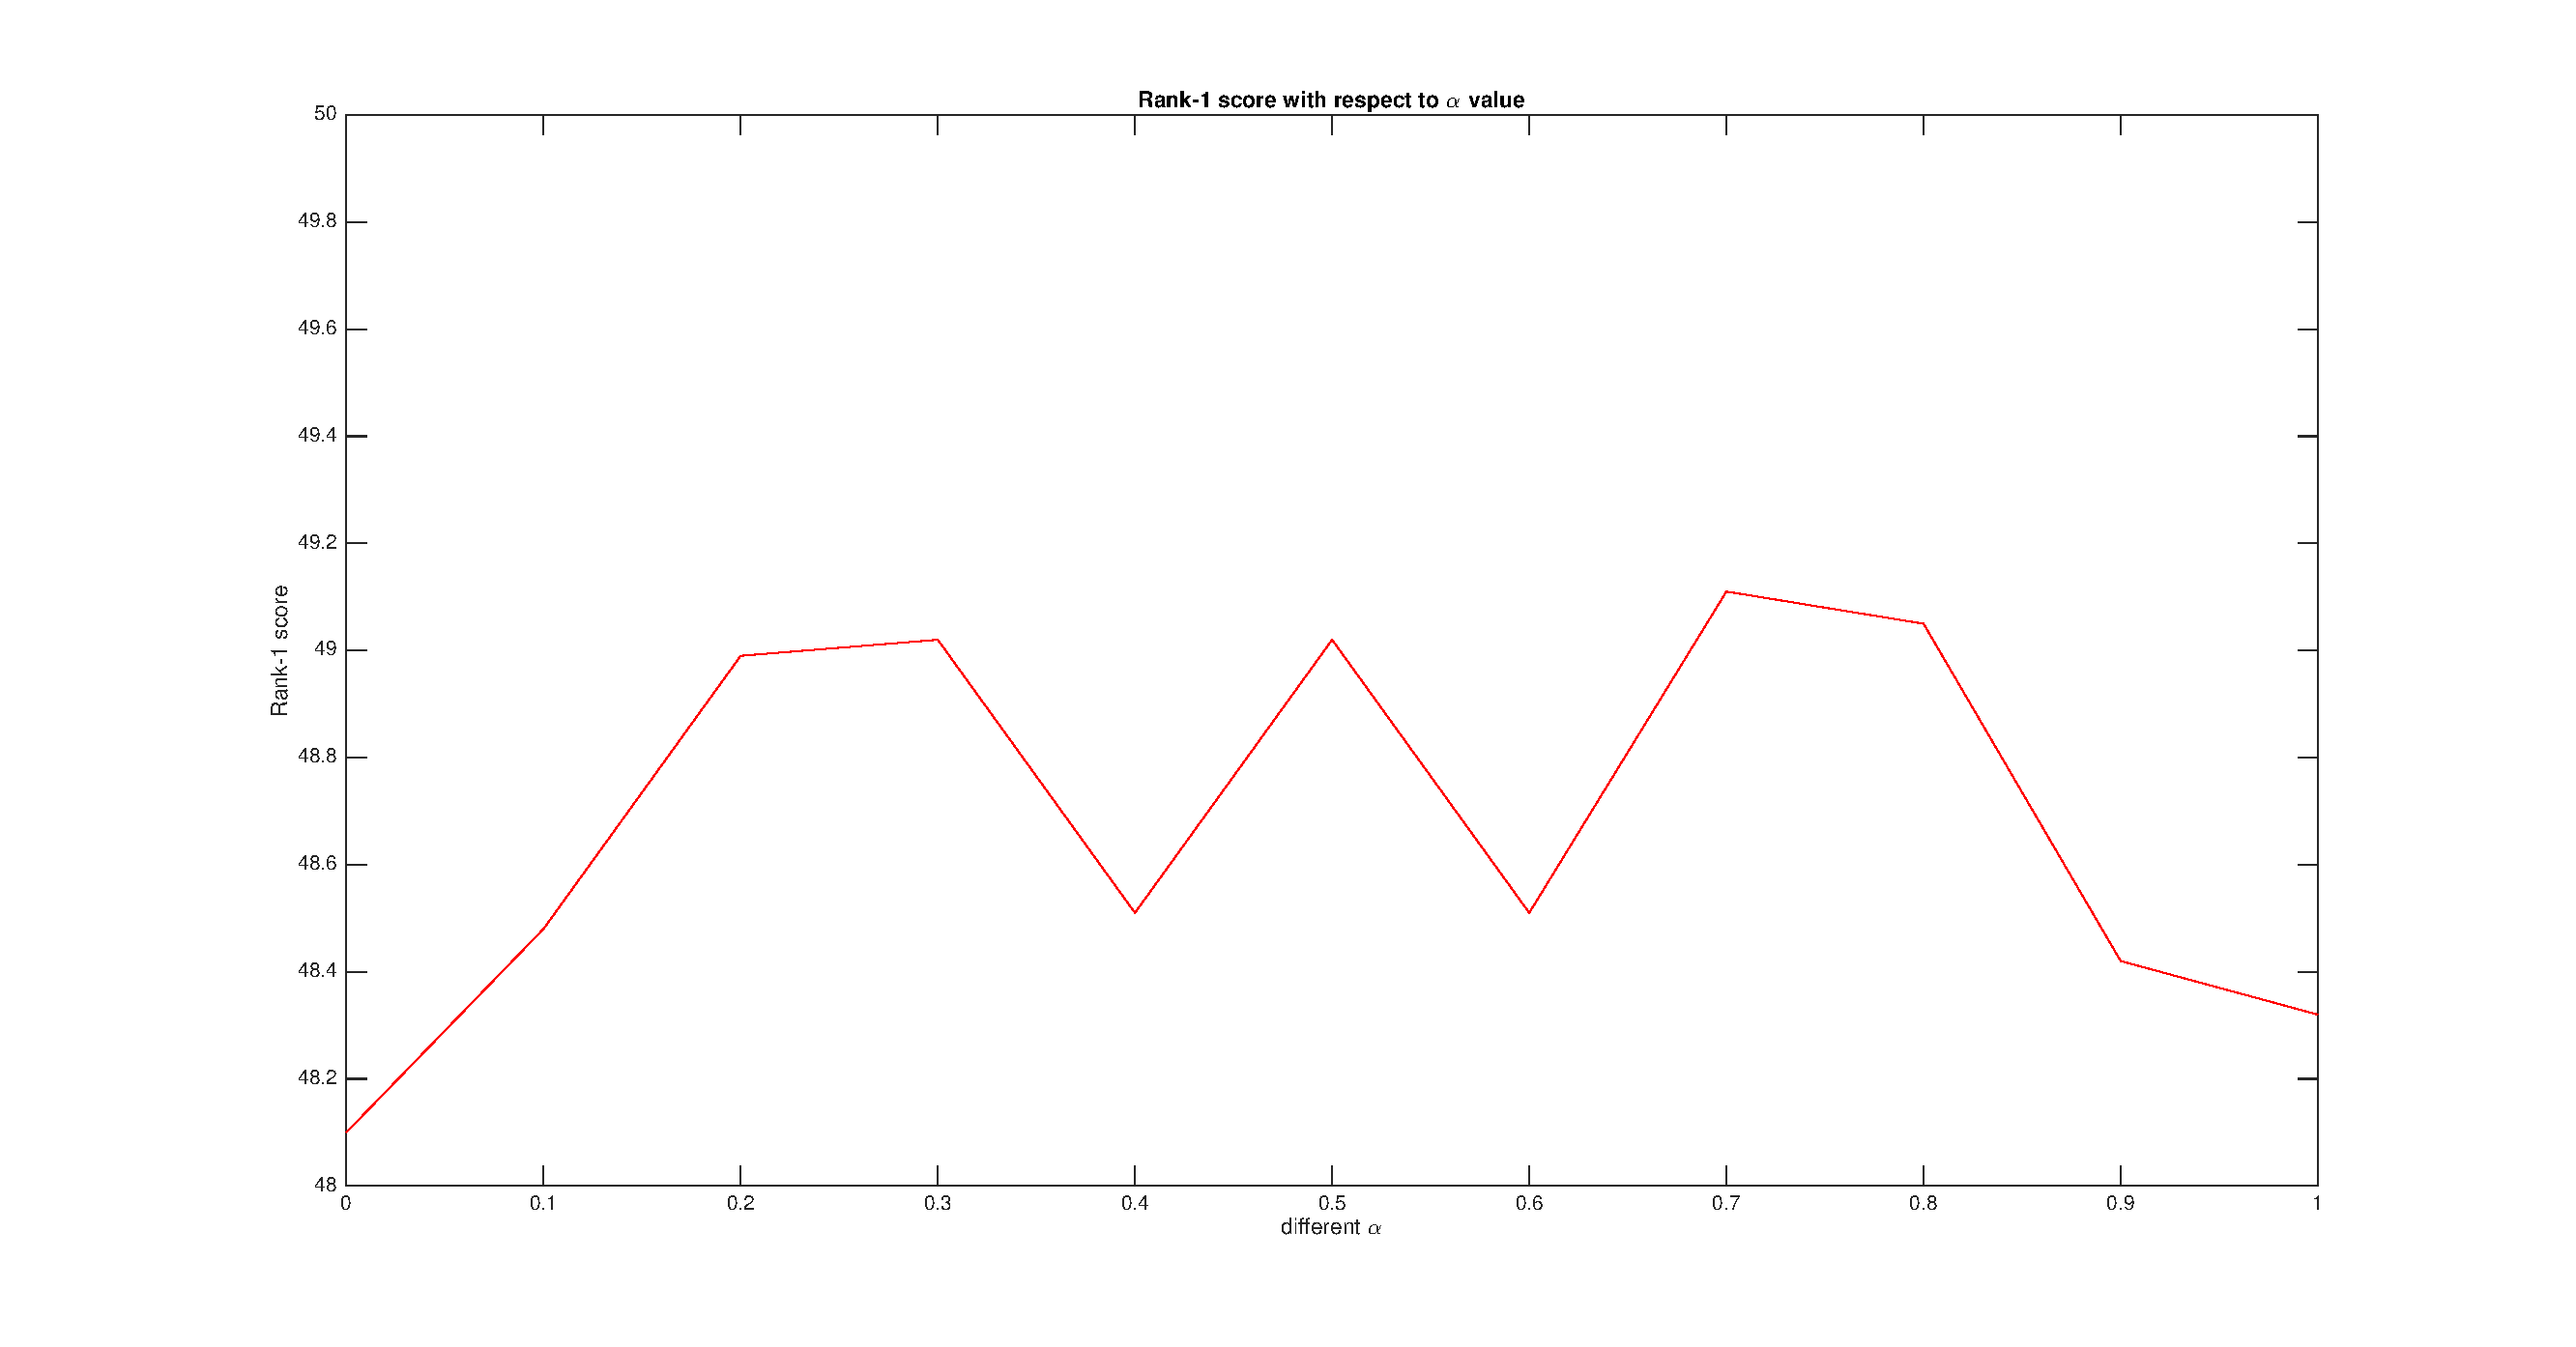
\includegraphics[width=1\linewidth]{Rank1scoresAlpha.eps}
%\vspace{-3em}
%\caption{Rank 1 scores with respect to $\alpha$ on VIPeR}
%\end{raggedleft}
%\end{figure}
%%-------------------------------------------------
%\begin{figure}
%\begin{raggedleft}
%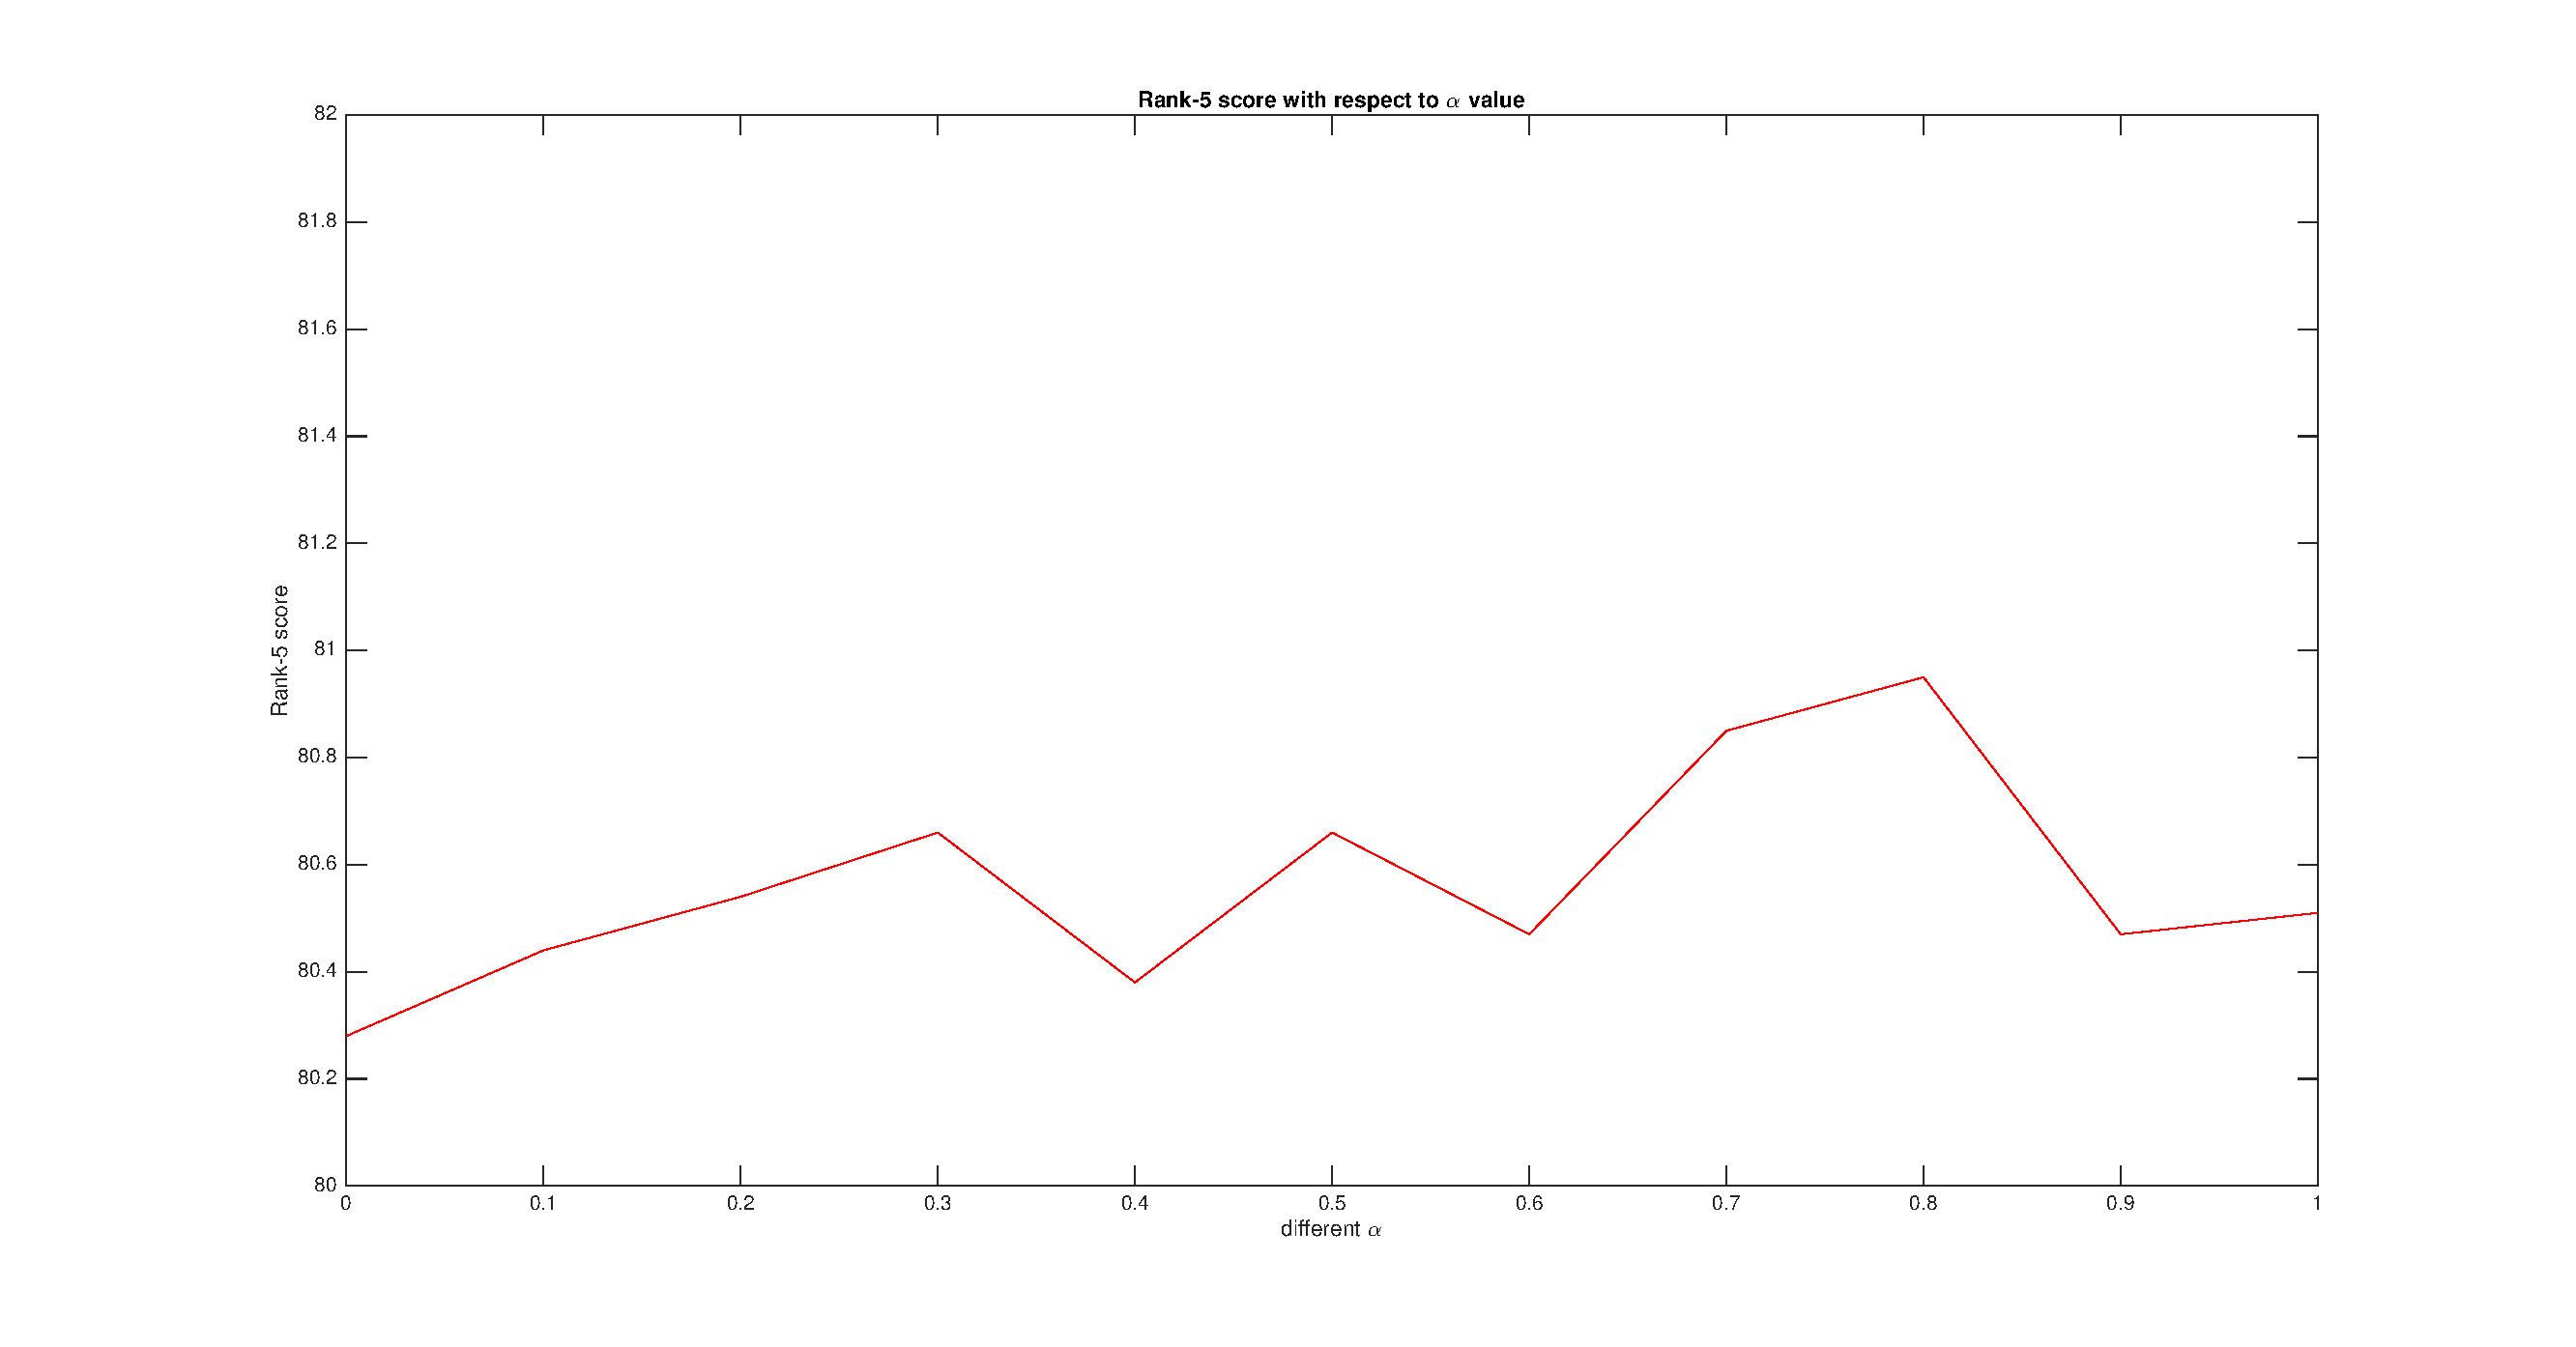
\includegraphics[width=1\linewidth]{Rank5scoresAlpha.eps}
%\vspace{-3em}
%\caption{Rank 5 scores with respect to $\alpha$ on VIPeR}
%\end{raggedleft}
%\end{figure}
%%-------------------------------------------------


\begin{table}[H]
\caption{Parameters setting}
\begin{tabular}{|l|c|c|c|c|c|}
\hline
Paramters &$\alpha$&thresh&step&Max iteration& slack variable\\
\hline
Values &0.76&$10^{-5}$&0.01&100&1\\
\hline
\end{tabular}
\end{table}


%\textbf{Performance measuring} The cumulative matching curve is used to measure the descriptor performance. The score means the probability that the right match is within the top $n$ samples. A perfect CMC curve is expected to have a high rank-1 value and reaches 1 as fast as possible.
\subsection{Performance analysis}
In this paper, we compare proposed metric with other state-of-the-art metrics including NFST \cite{NFST}, XQDA \cite{LOMO}. NFST is a metric which learn a null space for descriptors so that the the same class descriptors will be projected to  
a single point to minimize intraclass scatter matrix while different classes are projected to different points. This metric is a good solution to small sample problems in person re-identification. XQDA is quite similar with many other metrics, which learns a projection matrix $W$ and then a Mahanalobis SPD matrix $M$ is learned in the subspace. Those two metric are proved to have state-of-the-art performance compared with many other methods. The GOGrgb in all forms stands for the hierarchical gaussian descriptor in RGB color space while GOGfusion stands for the one in four different color spaces \{RGB, Lab, HSV, nRnG\}.\\
\textbf{VIPeR} A comparison form is given in Table 8. Some of recent results are also included in this form. We can find that the rank scores are better than those of NFST and XQDA in terms of both GOGrgb and GOGfusion. More specifically, the rank 1, rank 5, rank 10, rank 15 and rank 20 scores of proposed metric learning are 0.76\%, 0.92\%, 1.39\%, 1.08\%, 1.52\% higher than those of GOGrgb+XQDA, and the rank 1, rank 5, rank 10, rank 15 and rank 20 GOGfusion scores of proposed metric learning are 0.35\%, -0.54\%, 0.98\%, 0.66\%, 0.79\% higher than GOGfusion + XQDA respectively. Also we can see that the proposed metric learning has a better performance than NFST. \newline 
%-----------------------------------------------------------------------VIPeR
\begin{table}[H]
\caption{Performance of different metrics on VIPeR}
\centering
 \begin{tabular}{|l|c|c|c|c|c|c|}
\hline
& \multicolumn{5}{|c|}{Rank(\%)} \\
\hline
Methods& 1 & 5 &10& 15&20\\
\hline
GOGrgb+NFST& 43.23&73.16 &83.64 & 89.59&92.88\\  
\hline
GOGrgb+XQDA& 43.01&73.92&83.86& 89.24& 92.37\\
\hline
%GOGrgb+KLFDA&43.45 &74.68 &85.13 &90.54&93.70\\ 
%\hline
GOGrgb+Proposed&43.77 &74.84&85.25&90.32&93.89\\   %43.48%, 74.59%, 85.35%, 90.47%, 93.67%
\hline
GOGfusion+NFST&47.15& 76.39&87.31&91.74&94.49\\
\hline
GOGfusion+XQDA& 47.97& 77.44& 86.80& 91.27&93.70\\  
\hline
%GOGfusion+KLFDA & 47.97&77.06& 87.56&91.80&94.18\\
%\hline
GOGfusion+Proposed&48.32&76.90&87.78&91.93&94.49\\ %48.16%, 76.65%, 87.66%, 91.90%, 94.37% 
\hline

%--------------------------------------------------------------
\end{tabular}
\end{table}
\textbf{CUHK1} We can find that the rank 1, rank5, rank 10, rank 15, rank 20 score of GOGrgb combined with proposed metric are 5.4\%, 4.18\%,3.31\%,2.16\%,1.46\% higher than XQDA, and 0.31\%,1.22\%,1.34\%,1.17\%, 1.11\% than NFST.  Also the  rank 1, rank5, rank 10, rank 15, rank 20 score of GOGfusion combined with proposed metric are 4.57\%, 2.64\%, 0.70\%, 1.33\%, 0.83\% higher than GOGfusion combined with XQDA, and 0.41\%, 0.83\%, 0.88\%, 1.09\%, 1.14\% than GOGfusion combined with NFST. 

\begin{figure}
\begin{raggedleft}
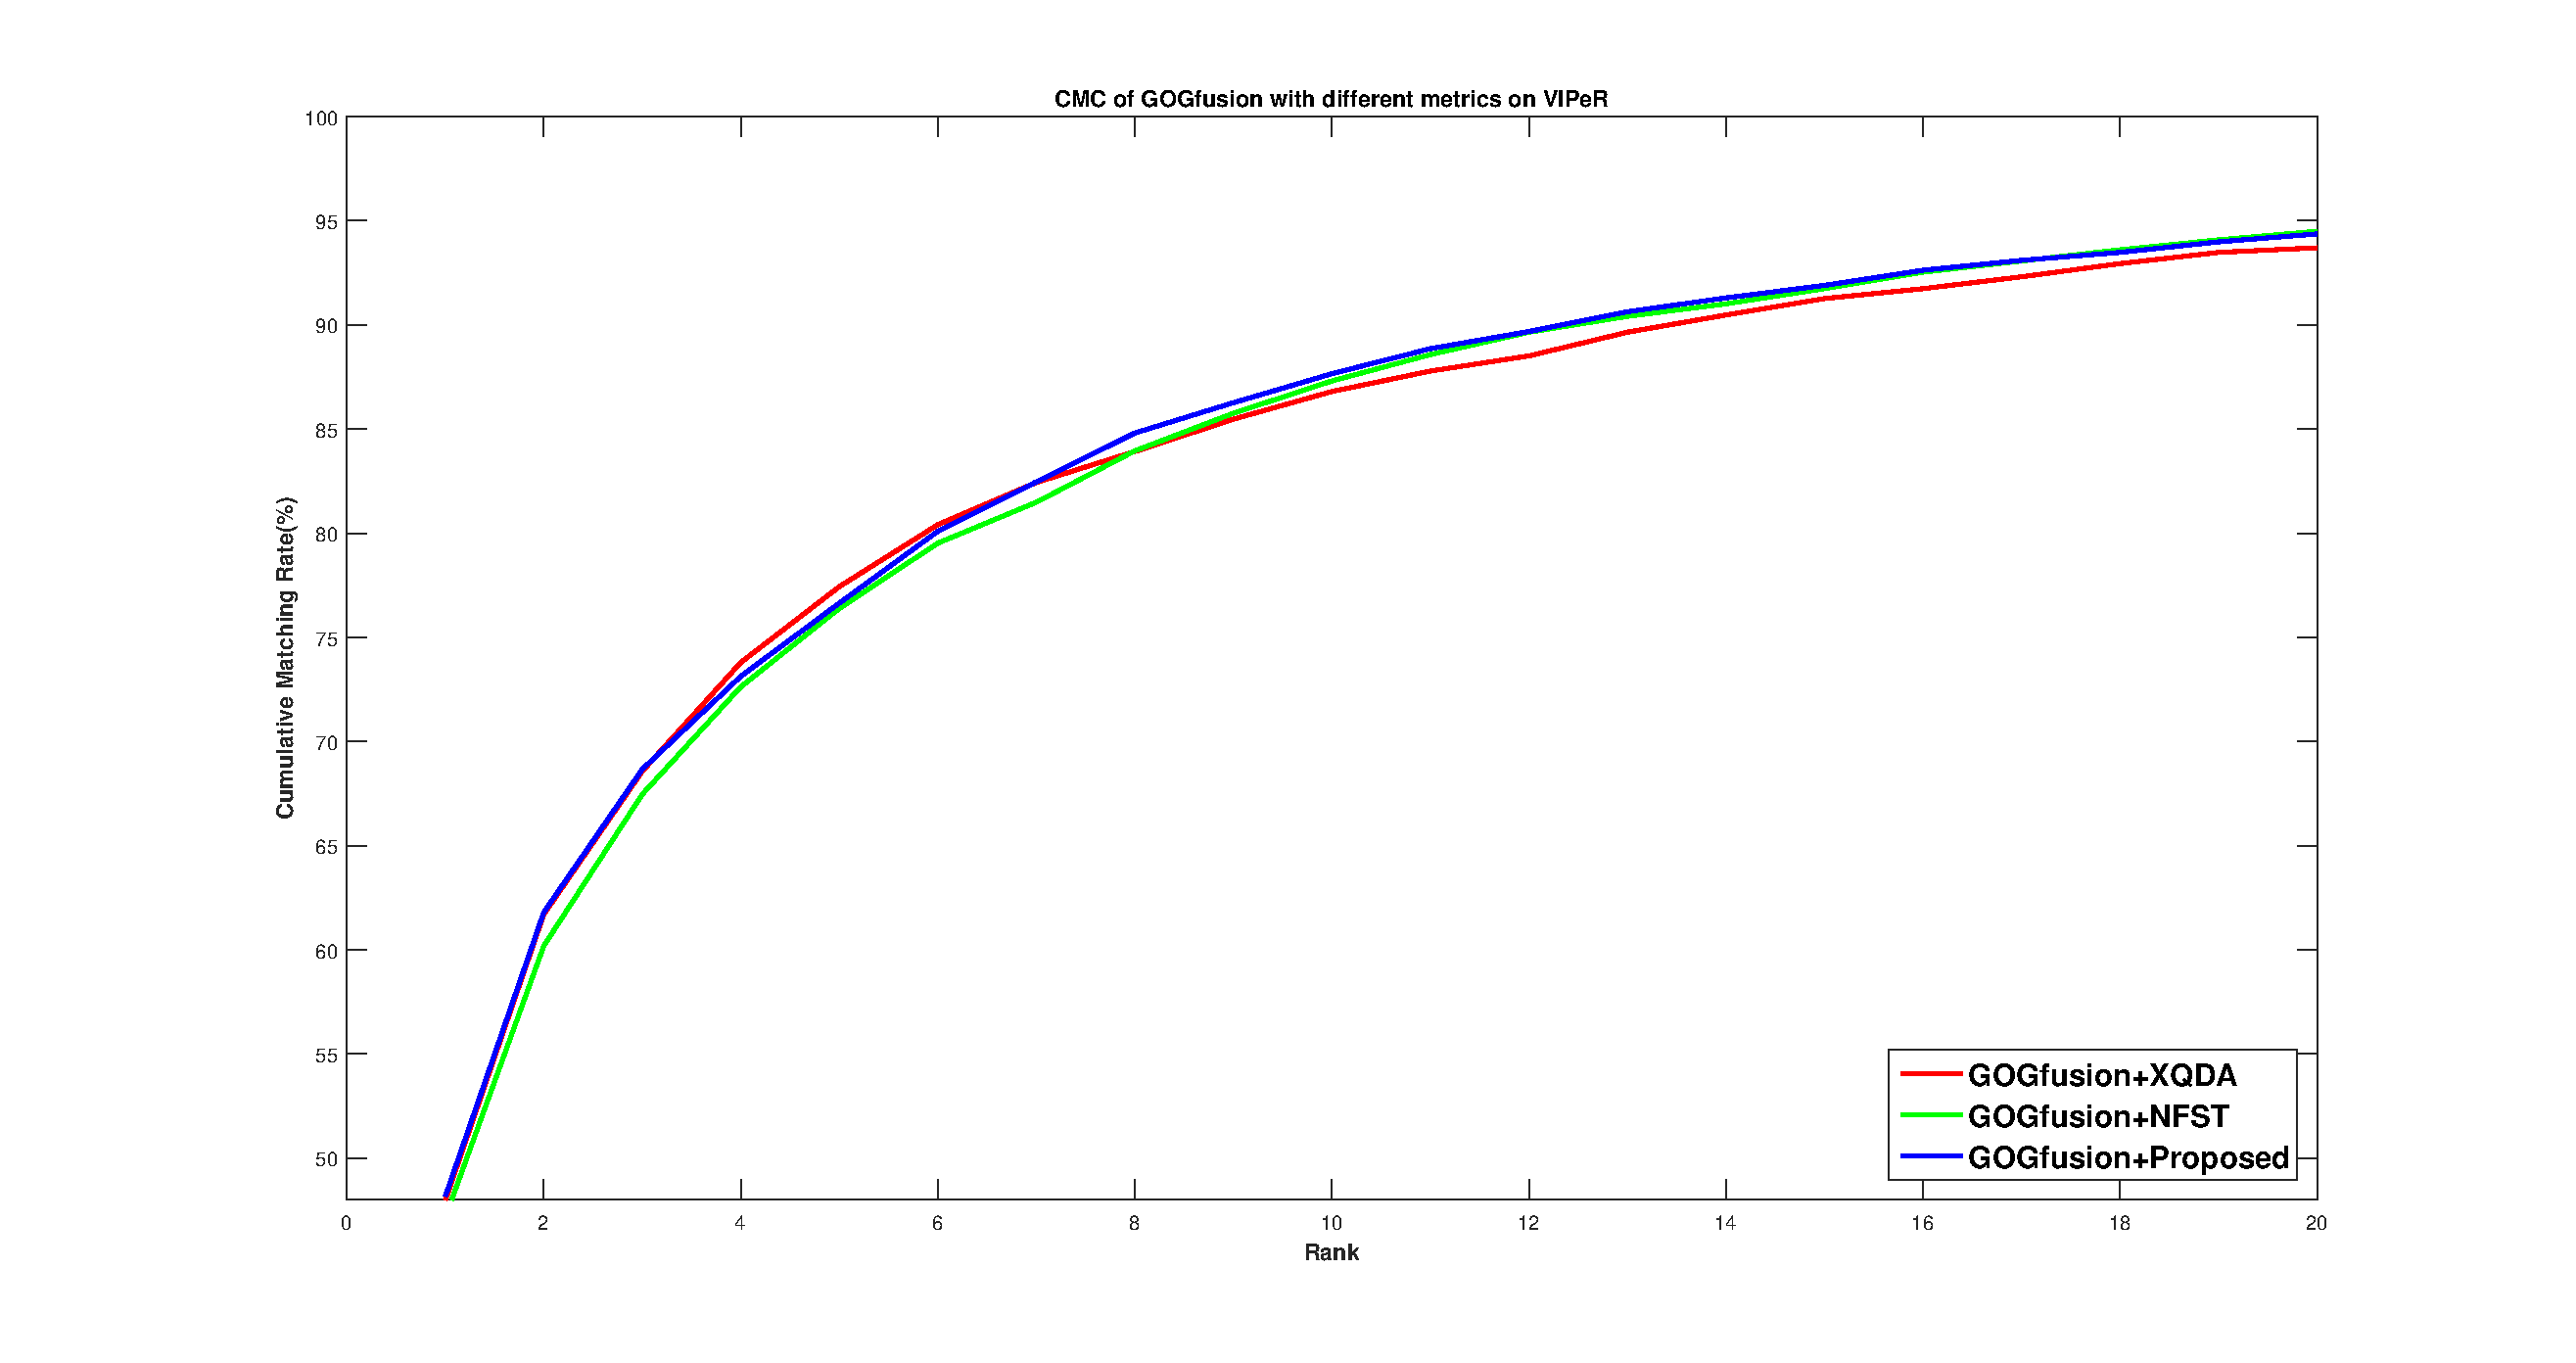
\includegraphics[width=1\linewidth]{VIPeR.eps}
\vspace{-3em}
\caption{CMC curves on VIPeR comparing different metric learning}
\end{raggedleft}
\end{figure}
%-------------------------------

%-----------------------------------------------------------------------CUHK1
\begin{table}[H]
\caption{Performance of different metrics on CUHK1}
\centering
\begin{tabular}{|l|c|c|c|c|c|c|}
\hline
& \multicolumn{5}{|c|}{Rank(\%)} \\
\hline
Methods& 1 & 5 &10&15& 20\\
\hline
GOGrgb+NFST&55.60 &83.02 &89.07 &91.98&93.56 \\ 
\hline
GOGrgb+XQDA&50.51 &80.06 &87.10 &90.99&93.21 \\ 
\hline
%GOGrgb+KLFDA&55.66&84.32&90.66&93.07& 94.63\\
%\hline
GOGrgb+Proposed&55.91&84.24&90.41& 93.15&94.67\\  %55.86%, 84.28%, 90.45%, 93.09%, 94.65% 
\hline
GOGfusion+NFST&56.26 &83.66 &89.63 &92.22&93.70 \\ 
\hline
GOGfusion+XQDA&52.10 &81.85&88.81 &91.98&94.01\\ 
\hline
%GOGfusion+KLFDA & 56.60&84.67&90.41&93.13&94.81\\
%\hline
GOGfusion+Proposed&56.67&84.49& 90.51& 93.31&94.84\\

\hline

\end{tabular}\newline
\end{table}

\begin{figure}
\begin{raggedleft}
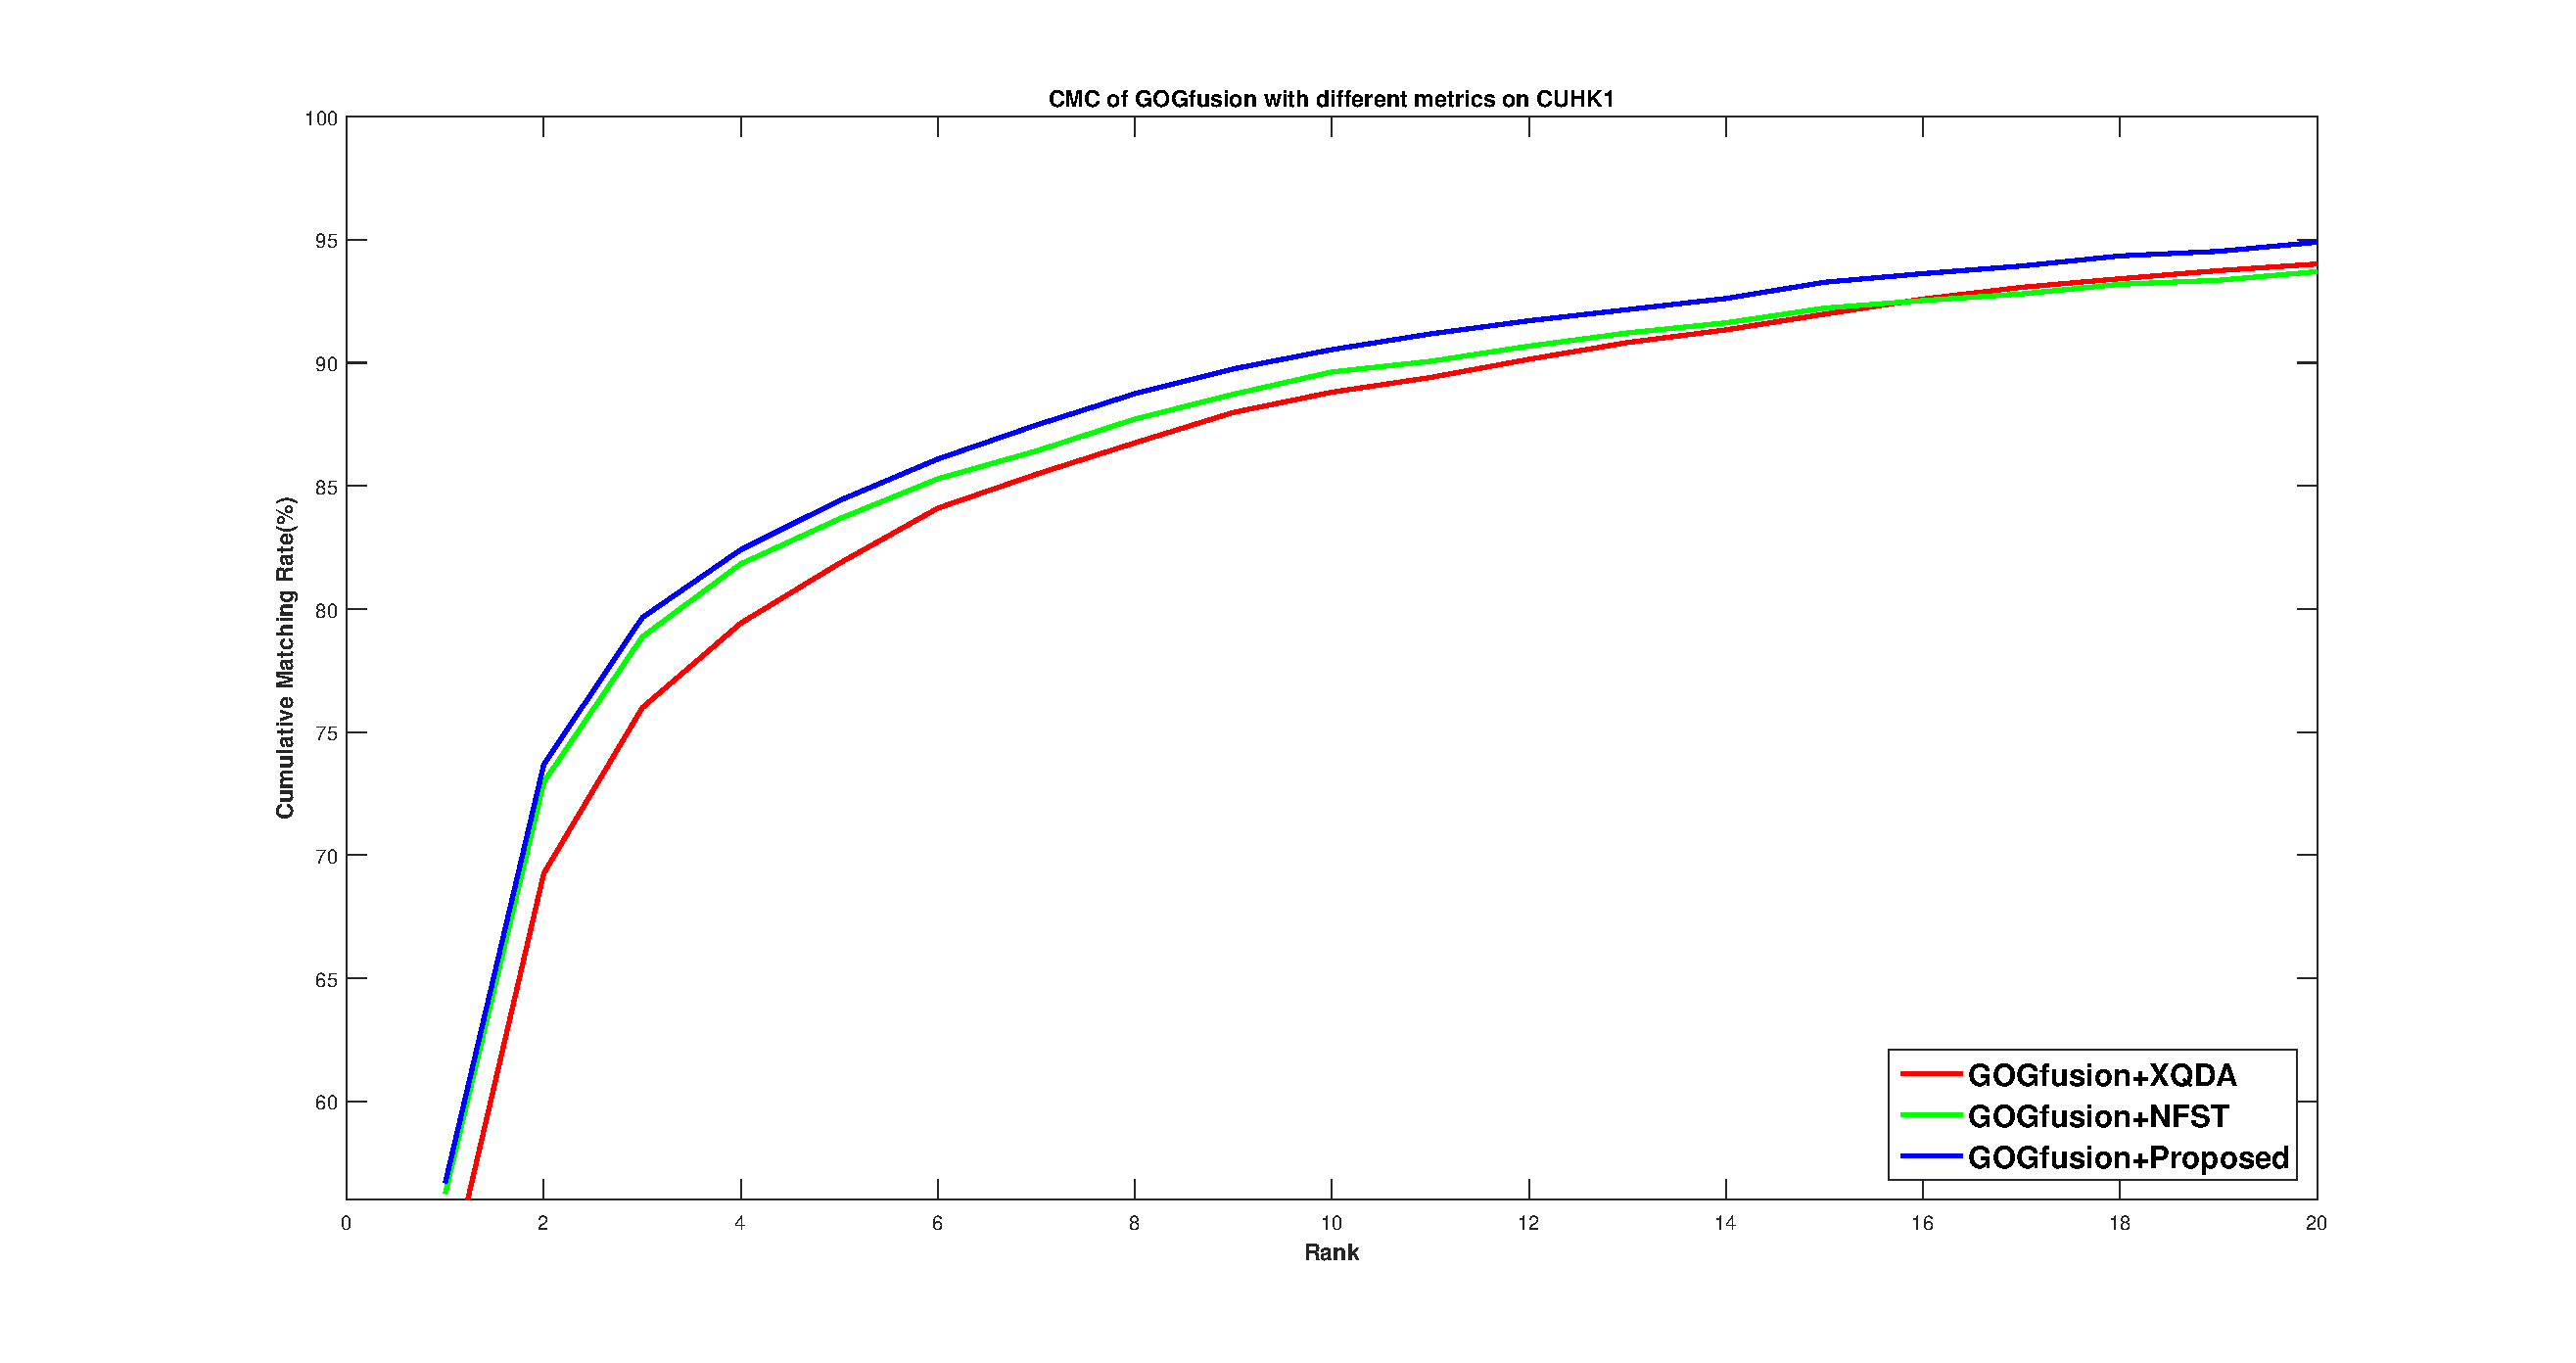
\includegraphics[width=1\linewidth]{CUHK1.eps}
\vspace{-3em}
\caption{CMC curves on CUHK1 comparing different metric learning}
\end{raggedleft}
\end{figure}

%-----------------------------------------------------------------------PRID_2011


\begin{table}[H]
\caption{Performance of different metrics on prid\_2011}
\centering
\begin{tabular}{|l|c|c|c|c|c|c|}
\hline
& \multicolumn{5}{|c|}{Rank(\%)} \\
\hline
Methods& 1 & 5 &10& 15&20\\
\hline
GOGrgb+NFST&26.60 &53.80& 62.90&71.30&75.40 \\ 
\hline
GOGrgb+XQDA&31.10 & 55.70& 66.10 & 72.40&76.10\\  
\hline
%GOGrgb+KLFDA&23.70&51.70&63.10&69.90&73.60\\ 
%\hline
GOGrgb+Proposed&23.80&52.20&63.50&70.20&73.50\\  %23.80%, 52.10%, 63.50%, 70.20%, 73.50%
\hline
GOGfusion+NFST&34.10 &58.30& 67.60&73.80&78.30 \\  
\hline
GOGfusion+XQDA&38.40& 61.30&70.80&75.60&79.30\\
\hline
%GOGfusion+KLFDA & 31.90&56.90&66.60&72.60&77.50\\
%\hline
GOGfusion+Proposed&32.30&57.40&66.30&73.40&78.00\\ %32.20%, 57.50%, 66.40%, 73.50%, 78.00(alpha = 0.7)   ()% 32.20%, 57.50%, 66.40%, 73.50%, 78.00%(alpha = 0.8)

\hline

\end{tabular}\newline
\end{table}
\textbf{Prid\_2011}  The  rank 1, rank5, rank 10, rank 15, rank 20 score of GOGfusion  combined with proposed metric are 6.1\%, 3.9\%, 4.5\%, 2.2\% and 1.3\% lower than GOGfusion combined with XQDA. The performance of NFST is slightly better than proposed metric. Also in terms of GOGrgb XQDA and NFST has better performance than the proposed one. So in this dataset the proposed metric has worse performance than XQDA and NFST.

\begin{figure}
\begin{raggedleft}
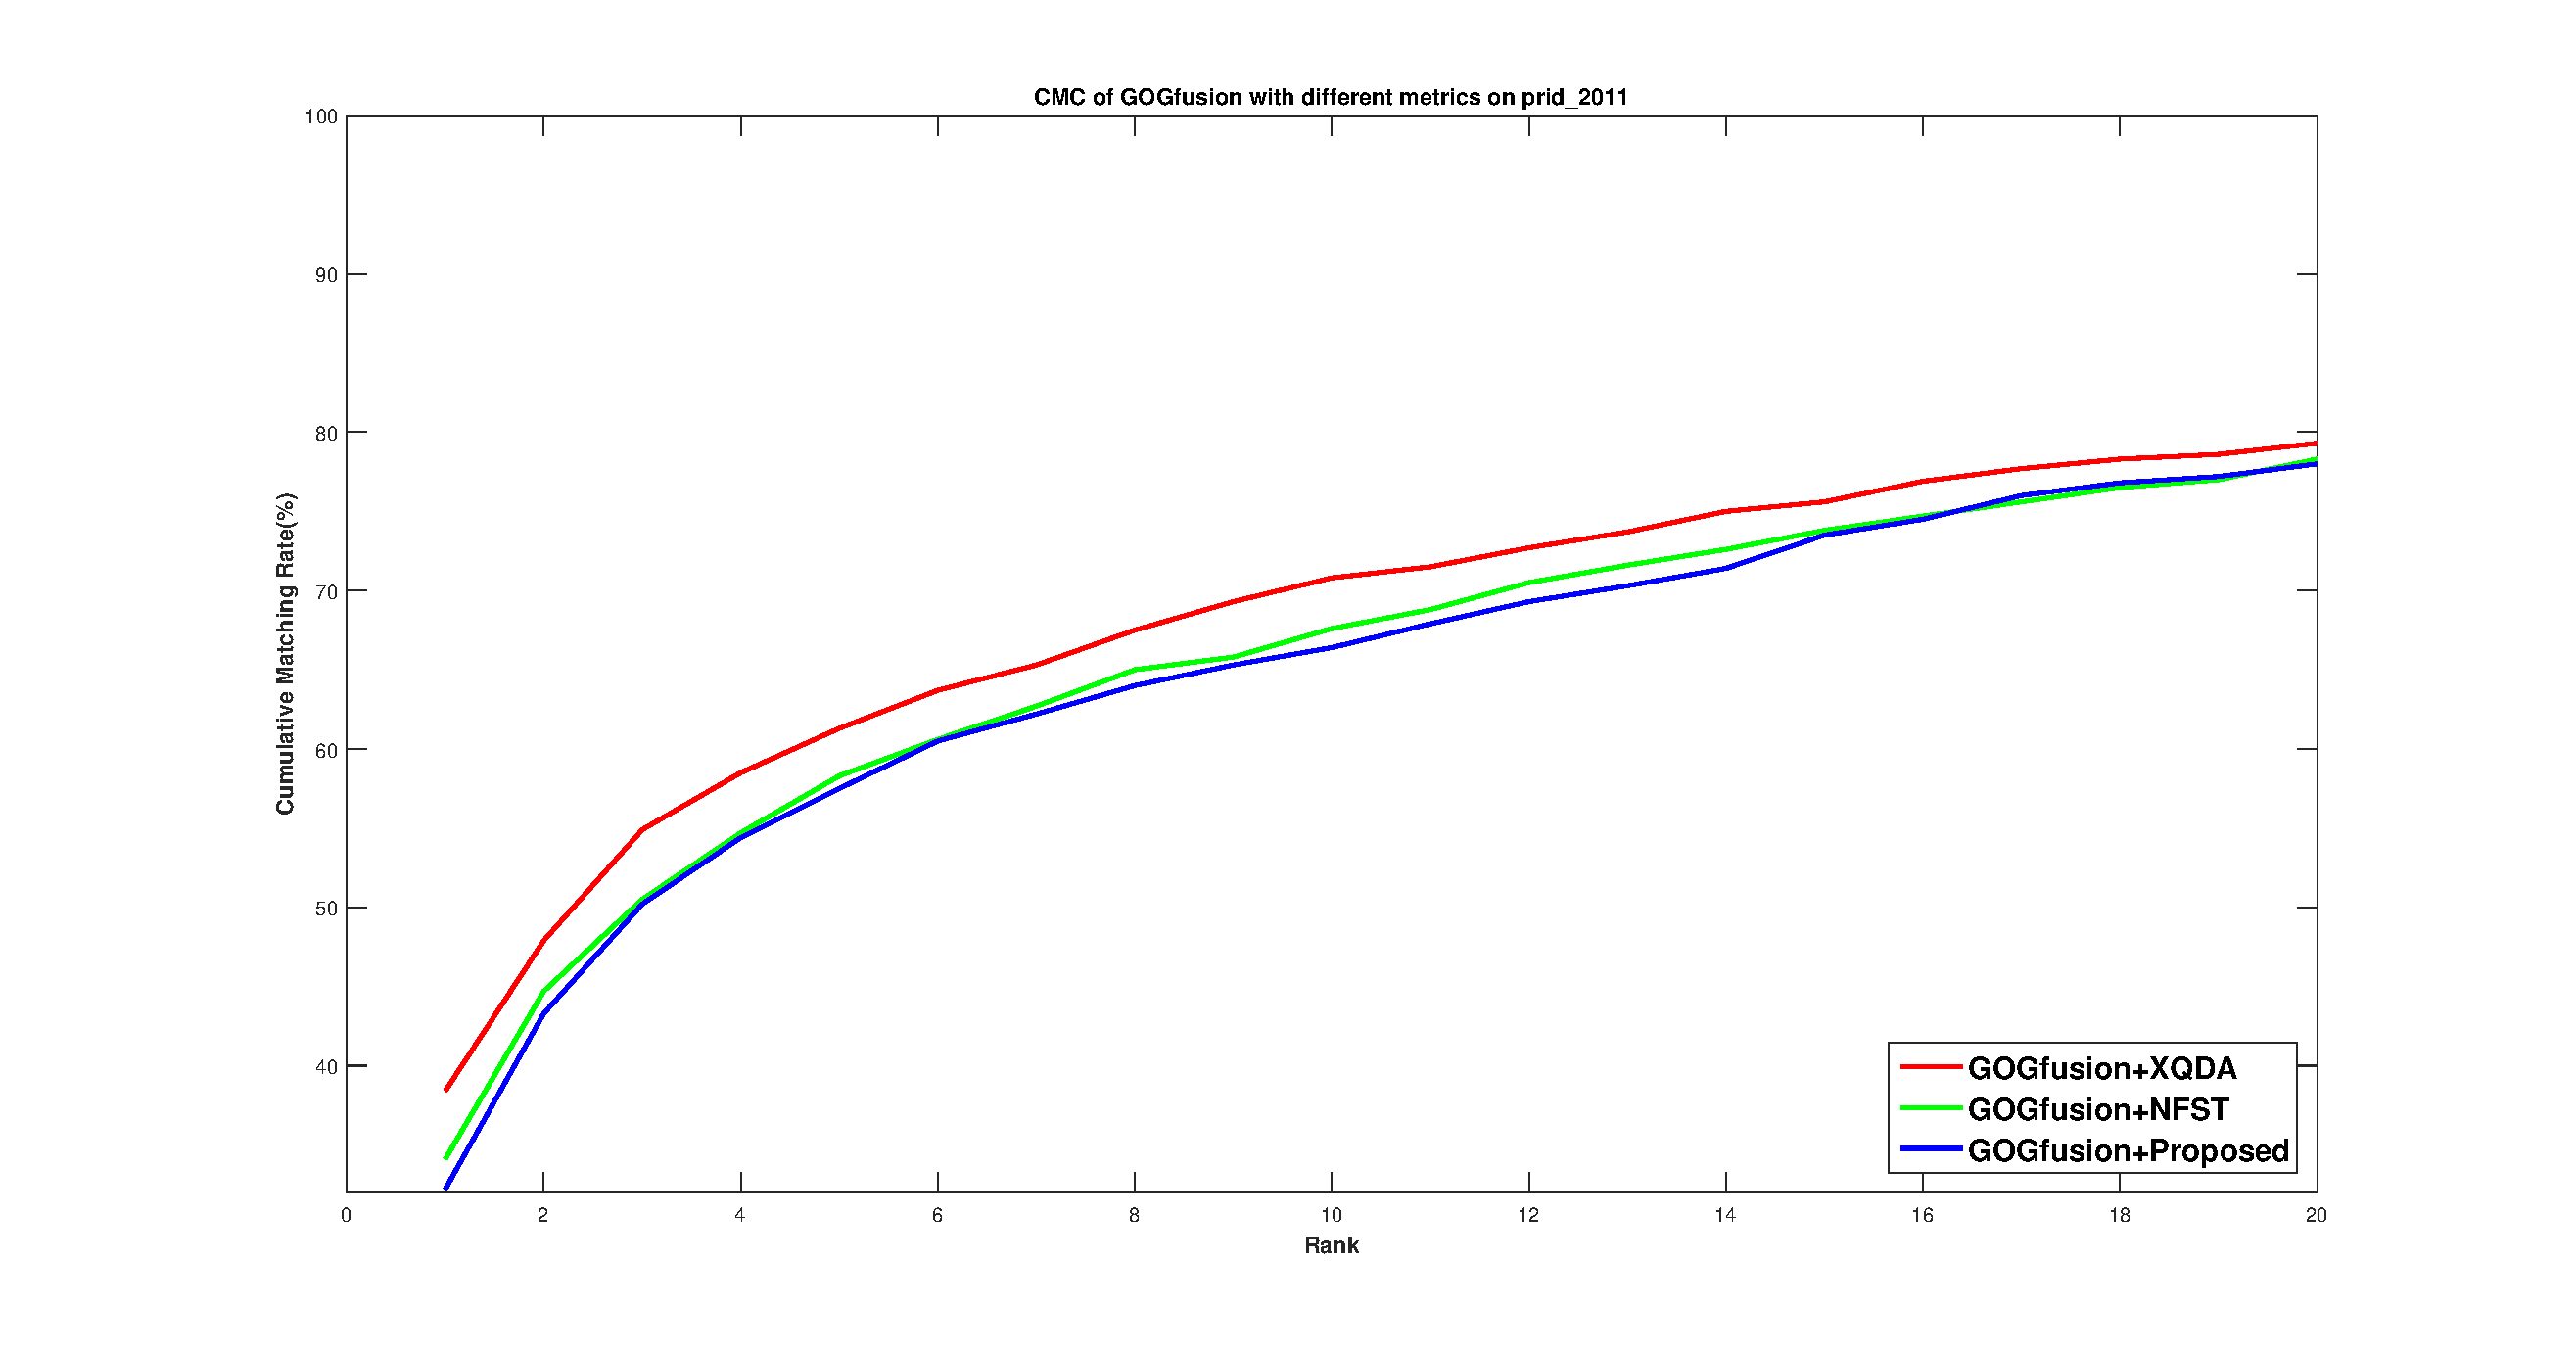
\includegraphics[width=1\linewidth]{prid2011.eps}
\vspace{-3em}
\caption{CMC curves on prid\_2011 comparing different metric learning}
\end{raggedleft}
\end{figure}

%-----------------------------------------------------------------------PRID_450S
\begin{table}[H]
\caption{Performance of different metrics on prid\_450s}
\centering
\begin{tabular}{|l|c|c|c|c|c|c|}
\hline
& \multicolumn{5}{|c|}{Rank(\%)} \\
\hline
Methods& 1 & 5 &10& 15&20\\
\hline
GOGrgb+NFST& 61.96&84.98 &90.53& 94.09&96.09 \\  %61.96%, 84.98%, 90.53%, 94.09%, 96.09%
\hline
GOGrgb+XQDA&65.29 &85.02 & 91.13&94.76& 96.49\\ 
\hline
%GOGrgb+KLFDA&60.04&84.09&90.93&94.04&96.00 \\ 
%\hline
GOGrgb+Proposed&60.71&84.53&91.29&94.13&96.27\\  %60.44%, 84.44%, 91.33%, 94.00%, 96.13%
\hline
GOGfusion+NFST& 64.53&86.62 & 92.93&95.78&97.42 \\ 
\hline
GOGfusion+XQDA&68.40 & 87.42&93.47 &95.69& 97.02\\ 
\hline
%GOGfusion+KLFDA & 62.58&86.18&92.18&95.11&96.84\\
%\hline
GOGfusion+Proposed&62.80&86.58&92.36&95.29& 96.89\\ % 62.62%, 86.44%, 92.36%, 95.20%, 96.93%(alpha = 0.7) 62.89%, 86.49%, 92.49%, 95.29%, 97.07%(alpha = 0.8)

\hline

\end{tabular}
\end{table}
\textbf{Prid\_450s} In this dataset, we can find the rank 1 score of XQDA and NFST is higher than proposed metric, but they have almost the same rank 5, rank 10, rank 15, and rank 20 scores with respect to both kinds of descriptors. 

\begin{figure}
\begin{raggedleft}
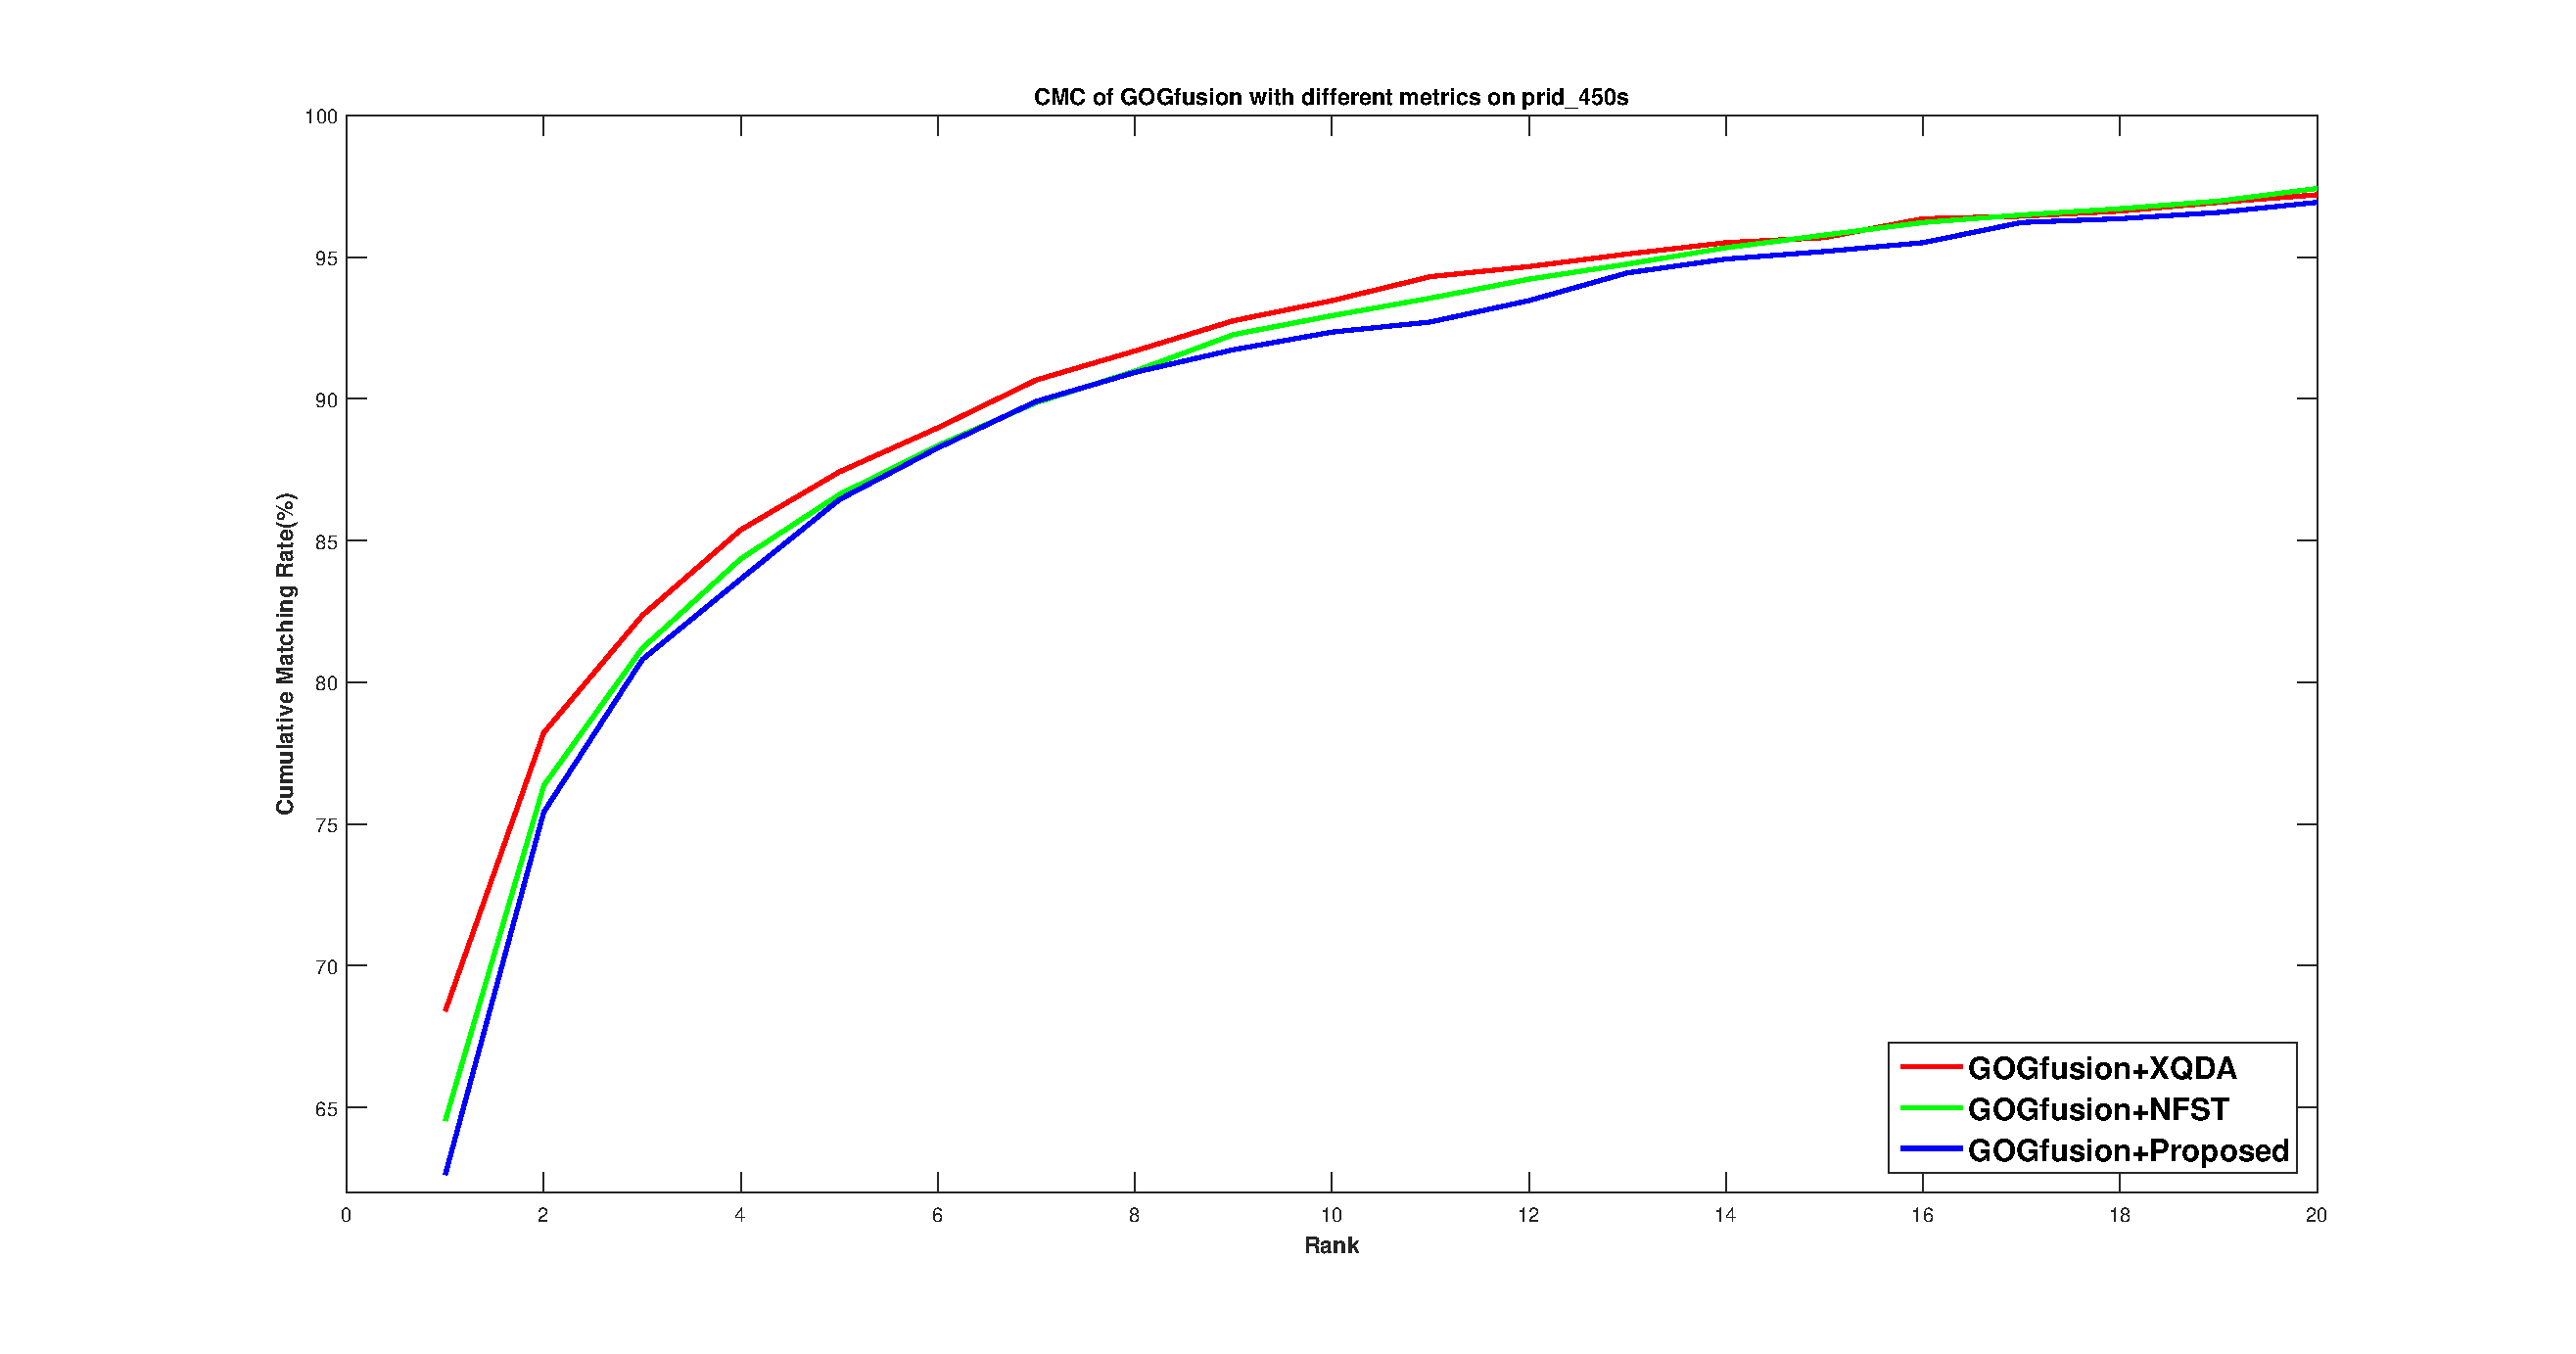
\includegraphics[width=1\linewidth]{prid450s.eps}
\vspace{-3em}
\caption{CMC curves on prid\_450s comparing different metric learning}
\end{raggedleft}
\end{figure}

%-----------------------------------------------------------------------GRID
\begin{table}[H]
\caption{Performance of different metrics on GRID}
\centering
\begin{tabular}{|l|c|c|c|c|c|c|}
\hline
& \multicolumn{5}{|c|}{Rank(\%)} \\
\hline
Methods& 1 & 5 &10& 15&20\\
\hline
GOGrgb+NFST& 21.84&41.28 &50.96& 57.44&62.88 \\ 
\hline
GOGrgb+XQDA& 22.64&43.92 &55.12 &61.12&66.56\\ 
\hline
%GOGrgb+KLFDA&23.44&43.04&52.16&59.12&64.88 \\ 
%\hline
GOGrgb+Proposed&22.64&43.68&52.00&59.04&65.04\\  %22.80%, 43.76%, 52.08%, 59.04%, 65.12%
\hline
GOGfusion+NFST& 23.04&44.40 &54.40 &61.84&66.56\\ 
\hline
GOGfusion+XQDA& 23.68&47.28 &58.40 &65.84&69.68 \\ 
\hline
%GOGfusion+KLFDA &23.76&44.40& 55.36&61.76& 66.48\\
%\hline
GOGfusion+Proposed&23.92&44.64&54.88&62.32&66.40\\ %23.84%, 44.64%, 55.04%, 62.24%, 66.24%

\hline

\end{tabular}
\end{table}

\begin{figure}
\begin{raggedleft}
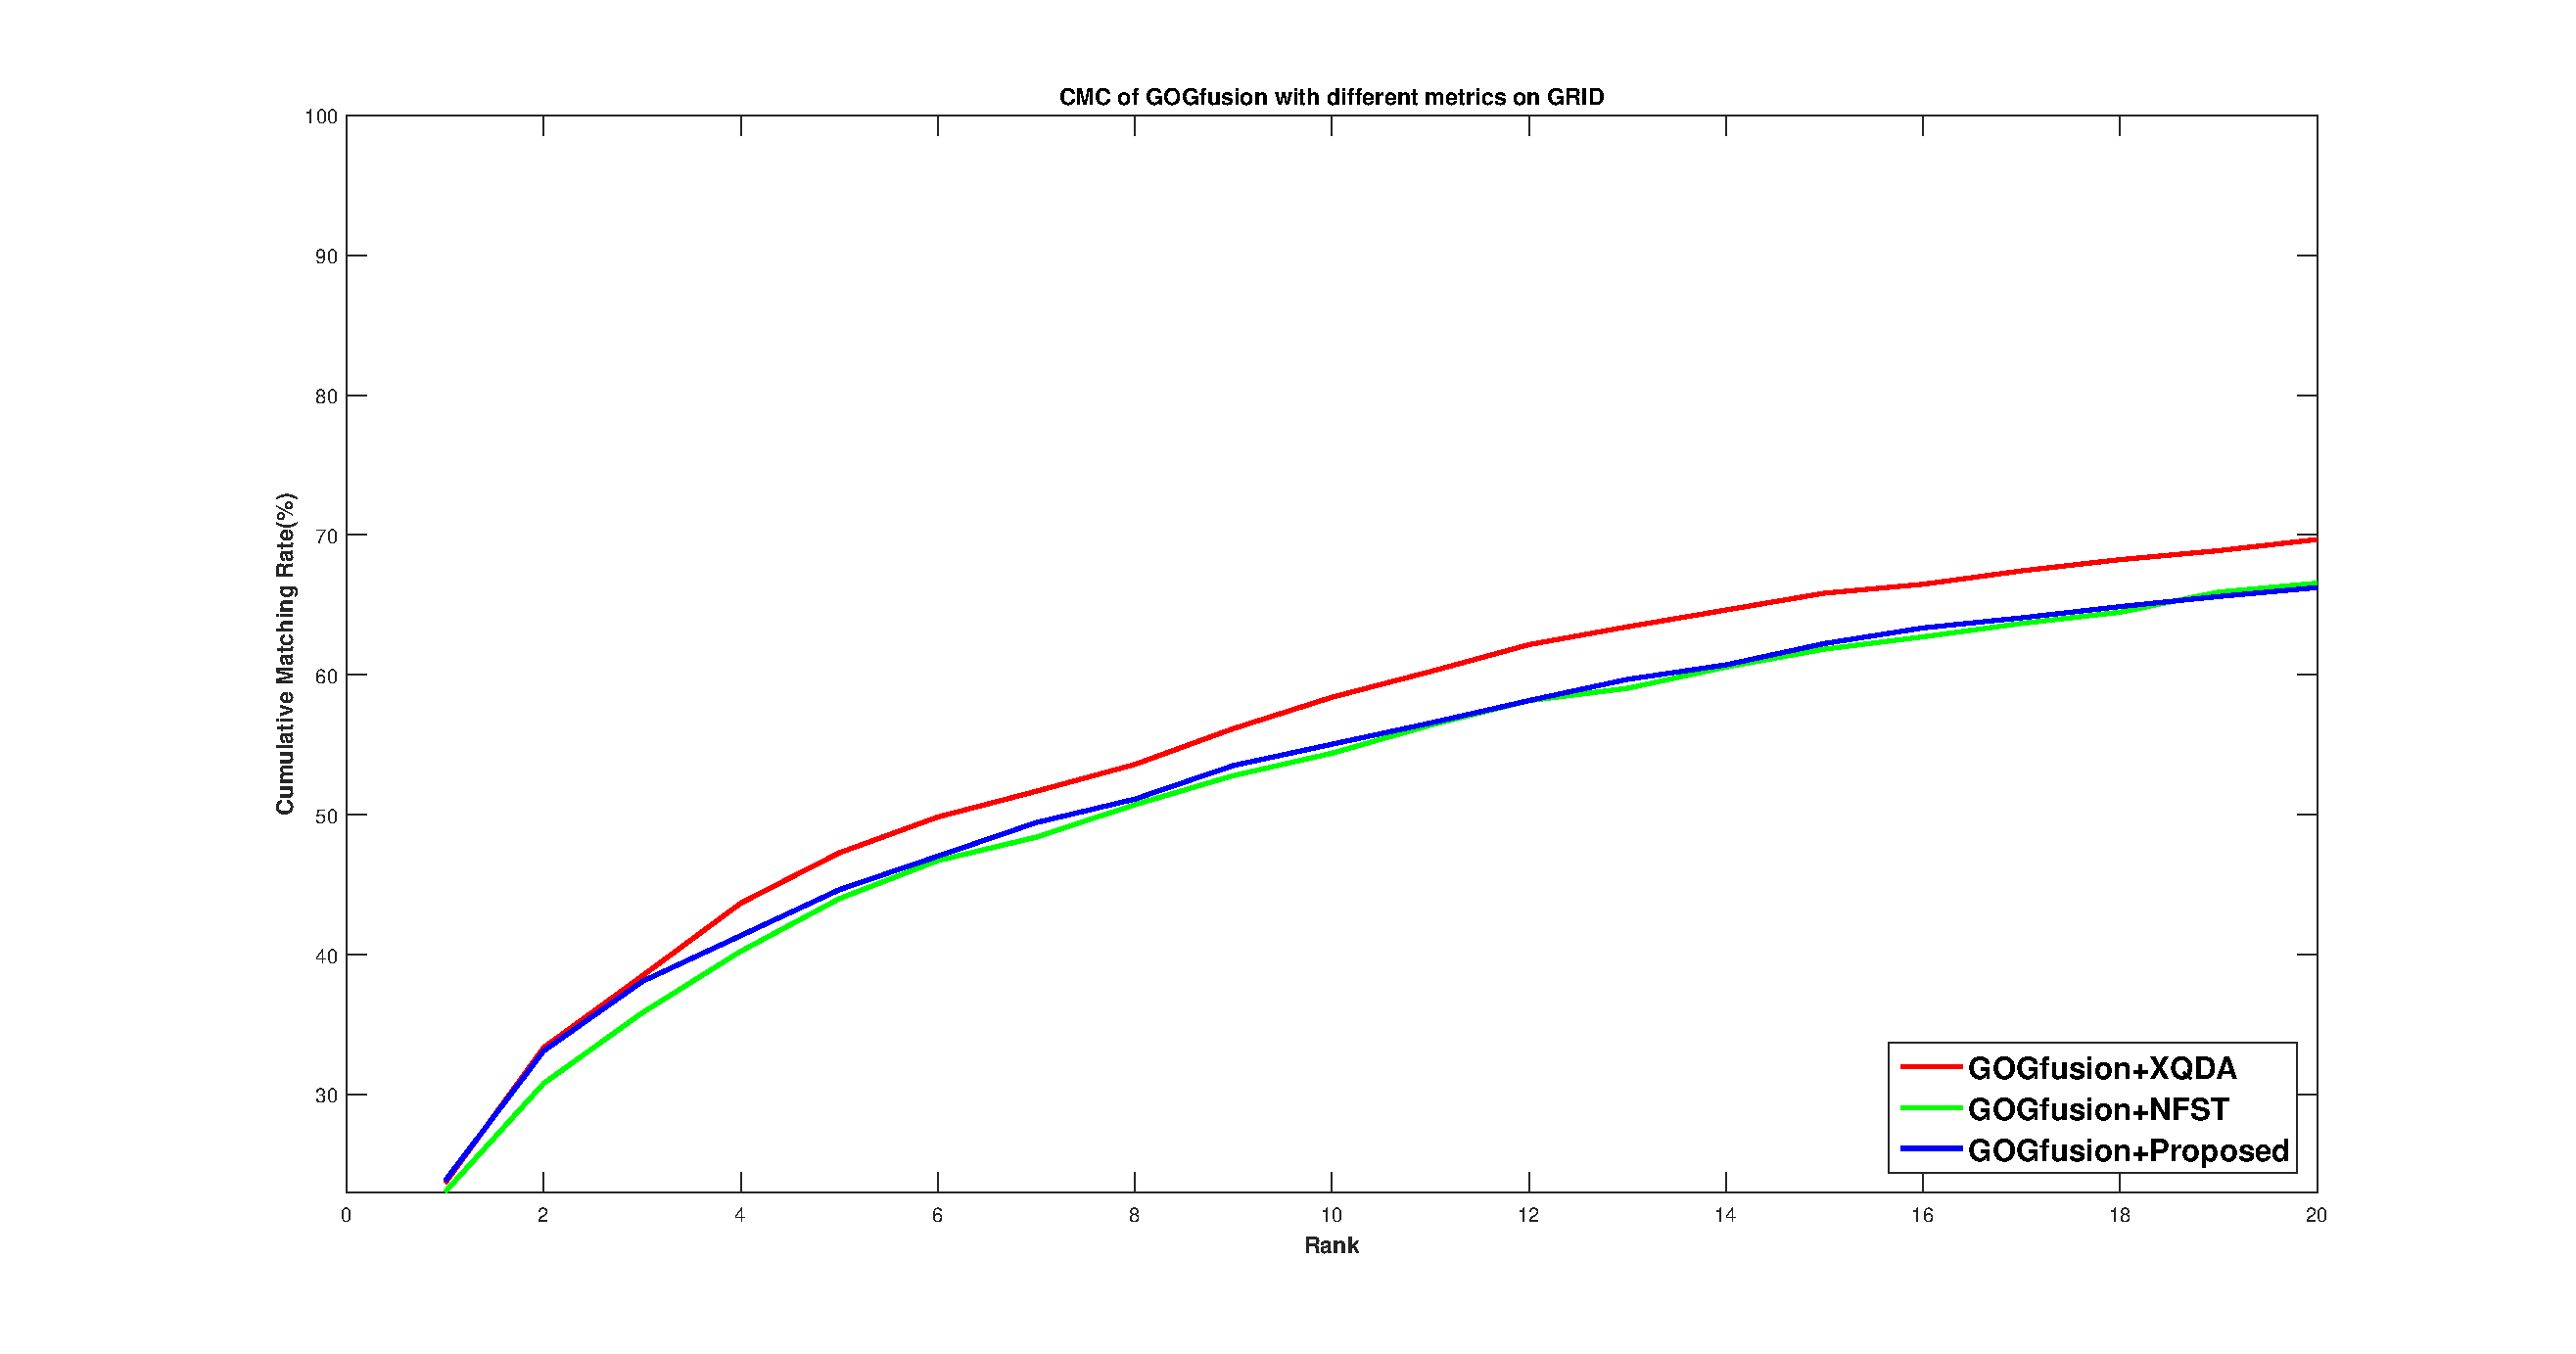
\includegraphics[width=1\linewidth]{GRID.eps}
\vspace{-3em}
\caption{CMC curves on GRID comparing different metric learning}
\end{raggedleft}
\end{figure}

\textbf{GRID} We can see that the rank 1 score of proposed metric are 0.24\% higher than XQDA and 0.88\% higher than NFST in terms of GOGfusion, but XQDA outperforms proposed metric on rank 5, rank 10, rank 15 and rank 20 scores. Besides, proposed metric outperforms NFST on rank 5, rank 10, rank 15 scores.


%------------------------------------------------------------------------

\section{Conclusion}
In this paper we combined KLFDA with gradient descent method based metric learning. A semi-positive definite(SPD) matrix is learned on the lower dimension space after dimension reduction by kernel local fisher discriminative analysis. By analysis we can find the proposed metric has better performance than NFST and XQDA on VIPeR and CUHK1 datasets, but XQDA and NFST outperforms the proposed metric learning on Prid\_2011 and Prid\_450s, and the proposed metric learning has better rank 1 score than NFST and its performance is only second to XQDA on GRID dataset.

% conference papers do not normally have an appendix

% use section* for acknowledgment
%\ifCLASSOPTIONcompsoc
%  % The Computer Society usually uses the plural form
%  \section*{Acknowledgments}
%\else
%  % regular IEEE prefers the singular form
%  \section*{Acknowledgment}
%\fi
%
%
%The authors would like to thank...
%




% trigger a \newpage just before the given reference
% number - used to balance the columns on the last page
% adjust value as needed - may need to be readjusted if
% the document is modified later
%\IEEEtriggeratref{8}
% The "triggered" command can be changed if desired:
%\IEEEtriggercmd{\enlargethispage{-5in}}

% references section

% can use a bibliography generated by BibTeX as a .bbl file
% BibTeX documentation can be easily obtained at:
% http://mirror.ctan.org/biblio/bibtex/contrib/doc/
% The IEEEtran BibTeX style support page is at:
% http://www.michaelshell.org/tex/ieeetran/bibtex/
%\bibliographystyle{IEEEtran}
% argument is your BibTeX string definitions and bibliography database(s)
%\bibliography{IEEEabrv,../bib/paper}
%
% <OR> manually copy in the resultant .bbl file
% set second argument of \begin to the number of references
% (used to reserve space for the reference number labels box)

\bibliographystyle{IEEEtran}
\bibliography{citation}
%\begin{thebibliography}{50}
%\bibitem{}
%\end{thebibliography}


% that's all folks
\end{document}



